\part{Quantum Spins, Coherent-state Path Integral, and Topological Terms}

\chapter{Quantum Spin}

We begin by considering the Hilbert space $\hilbert$ for a single quantum spin-1/2 particle. This is a two-dimensional complex vector space.

The conventional approach is to use an orthonormal basis formed by the eigenvectors of the spin operator along a chosen axis, typically the $z$-axis, denoted $\op{S}_z$.
\begin{equation}
    \op{S}_z \ket{\uparrow} = +\frac{\hbar}{2} \ket{\uparrow} \quad \text{and} \quad \op{S}_z \ket{\downarrow} = -\frac{\hbar}{2} \ket{\downarrow}
\end{equation}
Here, $\ket{\uparrow}$ represents the "spin up" state and $\ket{\downarrow}$ represents the "spin down" state. These two states form a complete orthonormal basis, satisfying:
\begin{itemize}
    \item \textbf{Orthogonality:} $\braket{\uparrow}{\downarrow} = 0$
    \item \textbf{Normalization:} $\braket{\uparrow}{\uparrow} = \braket{\downarrow}{\downarrow} = 1$
    \item \textbf{Completeness:} $\ketbra{\uparrow}{\uparrow} + \ketbra{\downarrow}{\downarrow} = \opI$
\end{itemize}
where $\opI$ is the identity operator in $\hilbert$.

But this simple, discrete basis has two drawbacks:
\begin{itemize}
    \item This discrete parametrized complete-set 
    is not convenient for constructing the path integral formalism of quantum spins.
    \item $SU(2)$ spin symmetry is broken either explicitly or not manifest.
\end{itemize}

\section{Spin Coherent States}

A general, normalized state $\ket{\psi}$ in the spin-1/2 Hilbert space can be written as a complex linear combination of the basis states:
\begin{equation}
    \ket{\psi} = z_1 \ket{\uparrow} + z_2 \ket{\downarrow}
\end{equation}
where $z_1, z_2 \in \mathbb{C}$ are complex coefficients.

The normalization condition $\braket{\psi}{\psi} = 1$ imposes a constraint on these coefficients:
\begin{equation}
    \bra{\psi}\psi\rangle = (|z_1|^2 + |z_2|^2) = 1
\end{equation}
A complex number $z = x + \mi y$ has two real parameters. Therefore, the pair $(z_1, z_2)$ is defined by four real parameters. The normalization condition $|z_1|^2 + |z_2|^2 = 1$ removes one degree of freedom, leaving three.

Furthermore, in quantum mechanics, the overall phase of a state vector is unphysical. The states $\ket{\psi}$ and $\me^{\mi\gamma} \ket{\psi}$ (for any real $\gamma$) represent the same physical state (i.e., they belong to the same ray in Hilbert space). This "gauge freedom" removes one more degree of freedom.

This leaves $4 - 1 - 1 = 2$ real, physical degrees of freedom. This is a crucial observation: the state space of a spin-1/2 particle is topologically equivalent to the surface of a 2D sphere, which is also parameterized by two angles (like latitude and longitude).

We can explicitly parameterize $z_1$ and $z_2$ using two angles, $\theta$ and $\phi$, which will map directly to the surface of a sphere. A standard (but not unique) parametrization for the spin coherent state, labeled by a unit vector $\bm{n}$, is:
\begin{equation}
    \ket{\bm{n}} \equiv \ket{\theta, \phi} = \cos\left(\frac{\theta}{2}\right) \me^{-\mi\phi/2} \ket{\uparrow} + \sin\left(\frac{\theta}{2}\right) \me^{\mi\phi/2} \ket{\downarrow}
    \label{eq:coherent_state}
\end{equation}
Here, the spherical coordinate angles have the domains $\theta \in [0, \mpi]$ and $\phi \in [0, 2\mpi)$. We can easily verify that this state is normalized:
\begin{equation}
    \braket{\bm{n}}{\bm{n}} = \left|\cos\left(\frac{\theta}{2}\right) \me^{-\mi\phi/2}\right|^2 + \left|\sin\left(\frac{\theta}{2}\right) \me^{\mi\phi/2}\right|^2 = \cos^2\left(\frac{\theta}{2}\right) + \sin^2\left(\frac{\theta}{2}\right) = 1
\end{equation}
This set of states $\{\ket{\bm{n}}\}$ is continuously parameterized by the angles $(\theta, \phi)$, addressing the first drawback of the discrete basis.

\subsection{Physical Interpretation: The Bloch Sphere}

To understand the physical meaning of $\theta$ and $\phi$, we compute the expectation value of the vector spin operator $\vecS$ in the state $\ket{\bm{n}}$. We will set $\hbar = 1$ from here on for simplicity. The spin operator is $\vecS = \frac{1}{2}\vecsigma$, where $\vecsigma = (\op{\sigma}_x, \op{\sigma}_y, \op{\sigma}_z)$ is the vector of Pauli matrices:
\begin{equation}
    \op{\sigma}_x = \begin{pmatrix} 0 & 1 \\ 1 & 0 \end{pmatrix}, \quad
    \op{\sigma}_y = \begin{pmatrix} 0 & -\mi \\ \mi & 0 \end{pmatrix}, \quad
    \op{\sigma}_z = \begin{pmatrix} 1 & 0 \\ 0 & -1 \end{pmatrix}
\end{equation}
In the $\ket{\uparrow}, \ket{\downarrow}$ basis, $\ket{\bm{n}}$ is represented by the column vector:
\begin{equation}
    \ket{\bm{n}} = \begin{pmatrix} \cos(\theta/2) \, \me^{-\mi\phi/2} \\ \sin(\theta/2) \, \me^{\mi\phi/2} \end{pmatrix}
    \quad \implies \quad
    \bra{\bm{n}} = \begin{pmatrix} \cos(\theta/2) \, \me^{\mi\phi/2} & \sin(\theta/2) \, \me^{-\mi\phi/2} \end{pmatrix}
\end{equation}

\paragraph{Expectation value of $\op{S}_z$:}
\begin{equation}\begin{aligned}
    \langle \op{S}_z \rangle &= \bra{\bm{n}} \left(\frac{1}{2}\op{\sigma}_z\right) \ket{\bm{n}}
    = \frac{1}{2} \begin{pmatrix} \cos(\theta/2) \, \me^{\mi\phi/2} & \sin(\theta/2) \, \me^{-\mi\phi/2} \end{pmatrix}
      \begin{pmatrix} 1 & 0 \\ 0 & -1 \end{pmatrix}
      \begin{pmatrix} \cos(\theta/2) \, \me^{-\mi\phi/2} \\ \sin(\theta/2) \, \me^{\mi\phi/2} \end{pmatrix} \\
    &= \frac{1}{2} \left( \cos^2\left(\frac{\theta}{2}\right) - \sin^2\left(\frac{\theta}{2}\right) \right)
    = \frac{1}{2} \cos(\theta)
\end{aligned}\end{equation}

\paragraph{Expectation value of $\op{S}_x$:}
\begin{equation}\begin{aligned}
    \langle \op{S}_x \rangle &= \bra{\bm{n}} \left(\frac{1}{2}\op{\sigma}_x\right) \ket{\bm{n}}
    = \frac{1}{2} \begin{pmatrix} \dots \end{pmatrix}
      \begin{pmatrix} 0 & 1 \\ 1 & 0 \end{pmatrix}
      \begin{pmatrix} \dots \end{pmatrix} \\
    &= \frac{1}{2} \left( \cos(\theta/2)\sin(\theta/2) \me^{\mi\phi/2} \me^{\mi\phi/2} + \sin(\theta/2)\cos(\theta/2) \me^{-\mi\phi/2} \me^{-\mi\phi/2} \right) \\
    &= \frac{1}{2} \cos(\theta/2)\sin(\theta/2) \left( \me^{\mi\phi} + \me^{-\mi\phi} \right)
    = \left(\frac{1}{2} \sin\theta\right) \left(\frac{\me^{\mi\phi} + \me^{-\mi\phi}}{2}\right)
    = \frac{1}{2} \sin\theta \cos\phi
\end{aligned}\end{equation}

\paragraph{Expectation value of $\op{S}_y$:}
\begin{equation}\begin{aligned}
    \langle \op{S}_y \rangle &= \bra{\bm{n}} \left(\frac{1}{2}\op{\sigma}_y\right) \ket{\bm{n}}
    = \frac{1}{2} \begin{pmatrix} \dots \end{pmatrix}
      \begin{pmatrix} 0 & -\mi \\ \mi & 0 \end{pmatrix}
      \begin{pmatrix} \dots \end{pmatrix} \\
    &= \frac{1}{2} \left( \cos(\theta/2)(-\mi)\sin(\theta/2) \me^{\mi\phi/2} \me^{\mi\phi/2} + \sin(\theta/2)(\mi)\cos(\theta/2) \me^{-\mi\phi/2} \me^{-\mi\phi/2} \right) \\
    &= \frac{1}{2} \cos(\theta/2)\sin(\theta/2) \left( -\mi \me^{\mi\phi} + \mi \me^{-\mi\phi} \right)
    = \left(\frac{1}{2} \sin\theta\right) \left(\frac{\me^{\mi\phi} - \me^{-\mi\phi}}{2\mi}\right)
    = \frac{1}{2} \sin\theta \sin\phi
\end{aligned}\end{equation}

Combining these results, the expectation value of the spin vector is:
\begin{equation}
    \langle \vecS \rangle = \frac{1}{2} \left( \sin\theta \cos\phi, \; \sin\theta \sin\phi, \; \cos\theta \right)
\end{equation}
This is a vector of length $S=1/2$ pointing in the direction specified by the unit vector $\bm{n}$:
\begin{equation}
    \bm{n} = (\sin\theta \cos\phi, \sin\theta \sin\phi, \cos\theta)
\end{equation}
Thus, the state $\ket{\bm{n}}$ is the quantum state that "points" in the classical direction $\bm{n}$. This direction vector lives on the surface of a unit sphere, known as the \textbf{Bloch Sphere}.

This formalism treats all directions $\bm{n}$ on an equal footing, making the SU(2) rotational symmetry manifest. This addresses the second drawback of the discrete basis.

% \subsection{Coherent State as an Eigenvector}

The eigenvector equation:
\begin{equation}
    (\vecS \cdot \vecn) \ket{\bm{n}} = \frac{1}{2} \ket{\bm{n}}
\end{equation}
This equation signifies that the coherent state $\ket{\bm{n}}$ is, by definition, the "spin up" eigenvector of the spin operator projected along its own pointing direction $\vecn$, with the eigenvalue $+1/2$ (with $\hbar=1$).


\begin{proof}
    We first construct the operator $\vecS \cdot \vecn$ in matrix form:
    \begin{equation}\begin{aligned}
        \vecS \cdot \vecn &= \op{S}_x n_x + \op{S}_y n_y + \op{S}_z n_z \\
        &= \frac{1}{2} (\op{\sigma}_x n_x + \op{\sigma}_y n_y + \op{\sigma}_z n_z) \\
        &= \frac{1}{2} \left[ \begin{pmatrix} 0 & 1 \\ 1 & 0 \end{pmatrix} \sin\theta \cos\phi + \begin{pmatrix} 0 & -\mi \\ \mi & 0 \end{pmatrix} \sin\theta \sin\phi + \begin{pmatrix} 1 & 0 \\ 0 & -1 \end{pmatrix} \cos\theta \right] \\
        &= \frac{1}{2} \begin{pmatrix}
        \cos\theta & \sin\theta (\cos\phi - \mi \sin\phi) \\
        \sin\theta (\cos\phi + \mi \sin\phi) & -\cos\theta
        \end{pmatrix} \\
        &= \frac{1}{2} \begin{pmatrix}
        \cos\theta & \sin\theta \, \me^{-\mi\phi} \\
        \sin\theta \, \me^{\mi\phi} & -\cos\theta
        \end{pmatrix}
    \end{aligned}\end{equation}
    Now, we apply this operator to the coherent state vector $\ket{\bm{n}}$:
    \begin{equation}
        (\vecS \cdot \vecn) \ket{\bm{n}} = \frac{1}{2} \begin{pmatrix}
        \cos\theta & \sin\theta \, \me^{-\mi\phi} \\
        \sin\theta \, \me^{\mi\phi} & -\cos\theta
        \end{pmatrix}
        \begin{pmatrix}
        \cos(\theta/2) \, \me^{-\mi\phi/2} \\
        \sin(\theta/2) \, \me^{\mi\phi/2}
        \end{pmatrix}
    \end{equation}
    We compute the top and bottom components of the resulting vector separately.

    \textbf{Top component:}
    \begin{equation}\begin{aligned}
        & \frac{1}{2} \left[ \cos\theta \cos(\theta/2) \me^{-\mi\phi/2} + \sin\theta \me^{-\mi\phi} \sin(\theta/2) \me^{\mi\phi/2} \right] \\
        &= \frac{1}{2} \me^{-\mi\phi/2} \left[ \cos\theta \cos(\theta/2) + \sin\theta \sin(\theta/2) \right] \\
        &= \frac{1}{2} \me^{-\mi\phi/2} \left[ \cos(\theta - \theta/2) \right] \quad \text{(using } \cos(A-B) \text{ identity)} \\
        &= \frac{1}{2} \cos(\theta/2) \me^{-\mi\phi/2}
    \end{aligned}\end{equation}
    This is precisely $\frac{1}{2}$ times the top component of $\ket{\bm{n}}$.

    \textbf{Bottom component:}
    \begin{equation}\begin{aligned}
        & \frac{1}{2} \left[ \sin\theta \me^{\mi\phi} \cos(\theta/2) \me^{-\mi\phi/2} - \cos\theta \sin(\theta/2) \me^{\mi\phi/2} \right] \\
        &= \frac{1}{2} \me^{\mi\phi/2} \left[ \sin\theta \cos(\theta/2) - \cos\theta \sin(\theta/2) \right] \\
        &= \frac{1}{2} \me^{\mi\phi/2} \left[ \sin(\theta - \theta/2) \right] \quad \text{(using } \sin(A-B) \text{ identity)} \\
        &= \frac{1}{2} \sin(\theta/2) \me^{\mi\phi/2}
    \end{aligned}\end{equation}
    This is precisely $\frac{1}{2}$ times the bottom component of $\ket{\bm{n}}$.

    Combining both components, we have shown:
    \begin{equation}
        (\vecS \cdot \vecn) \ket{\bm{n}} = \frac{1}{2} \begin{pmatrix}
        \cos(\theta/2) \me^{-\mi\phi/2} \\
        \sin(\theta/2) \me^{\mi\phi/2}
        \end{pmatrix}
        = \frac{1}{2} \ket{\bm{n}}
    \end{equation}
    This completes the proof. 
\end{proof}


\subsection{Gauge Choice and Topological Singularities}

The parametrization in Eq. \eqref{eq:coherent_state} is not unique, and it hides a subtle topological problem.
\begin{itemize}
    \item \textbf{At the North Pole} ($\theta=0$): The direction $\bm{n}$ is $(0,0,1)$. The angle $\phi$ is ill-defined. Our formula gives $\ket{\theta=0} = \cos(0)\me^{-\mi\phi/2}\ket{\uparrow} + \sin(0)\dots = \me^{-\mi\phi/2} \ket{\uparrow}$. The state vector itself depends on the meaningless angle $\phi$. This is a \textbf{singularity}.
    \item \textbf{At the South Pole} ($\theta=\mpi$): The direction $\bm{n}$ is $(0,0,-1)$. Our formula gives $\ket{\theta=\mpi} = \cos(\mpi/2)\dots + \sin(\mpi/2)\me^{\mi\phi/2}\ket{\downarrow} = \me^{\mi\phi/2} \ket{\downarrow}$. This is also singular.
\end{itemize}
This is analogous to the problem of creating a flat map of the Earth: you cannot do so without singularities (e.g., at the poles) or cuts.

We can "fix" the singularity at one pole by making a $\phi$-dependent gauge choice (i.e., multiplying by an overall phase $\me^{\mi\gamma(\phi)}$).

\textbf{Choice 1: Regular at North Pole.}
Let's choose an overall phase $\gamma = \phi/2$. The new state, $\ket{\bm{n}}_N$, is:
\begin{equation}
    \ket{\bm{n}}_N = \me^{\mi\phi/2} \ket{\bm{n}} = \cos\left(\frac{\theta}{2}\right) \ket{\uparrow} + \sin\left(\frac{\theta}{2}\right) \me^{\mi\phi} \ket{\downarrow}
\end{equation}
\begin{itemize}
    \item At the North Pole ($\theta=0$): $\ket{\bm{n}}_N = \cos(0)\ket{\uparrow} + \sin(0)\dots = \ket{\uparrow}$. This is now regular and well-defined.
    \item At the South Pole ($\theta=\mpi$): $\ket{\bm{n}}_N = \cos(\mpi/2)\ket{\uparrow} + \sin(\mpi/2)\me^{\mi\phi}\ket{\downarrow} = \me^{\mi\phi}\ket{\downarrow}$. The singularity has been "pushed" to the South Pole.
\end{itemize}

\textbf{Choice 2: Regular at South Pole.}
Let's choose $\gamma = -\phi/2$. The new state, $\ket{\bm{n}}_S$, is:
\begin{equation}
    \ket{\bm{n}}_S = \me^{-\mi\phi/2} \ket{\bm{n}} = \cos\left(\frac{\theta}{2}\right) \me^{-\mi\phi} \ket{\uparrow} + \sin\left(\frac{\theta}{2}\right) \ket{\downarrow}
\end{equation}
This state is regular at the South Pole ($\ket{\bm{n}}_S = \ket{\downarrow}$) but singular at the North Pole.

This unavoidable singularity is topological in nature and is the origin of the \textbf{Berry Phase}, or the "topological term," in the coherent-state path integral.

\subsection{Over-Completeness and Orthogonality}

The set of all coherent states $\{\ket{\bm{n}}\}$ for all $\bm{n}$ on the sphere is an \textbf{over-complete} basis. The Hilbert space is only 2-dimensional, but we have an infinite, continuous set of states. This means the states are not, in general, orthogonal.
\begin{equation}
    \braket{\bm{n}'}{\bm{n}} \neq 0 \quad \text{for } \bm{n}' \neq \bm{n} \text{ and } \bm{n}' \neq -\bm{n}
\end{equation}
A special exception, as noted in the text, is for antipodal states.

\subsection{Orthogonality of Antipodal States}
Let us prove that $\braket{-\bm{n}}{\bm{n}} = 0$. The antipodal point $-\bm{n}$ corresponds to the angles $(\theta', \phi') = (\mpi - \theta, \phi + \mpi)$.

We write the state $\ket{-\bm{n}}$ using Eq. \eqref{eq:coherent_state}:
\begin{equation}\begin{aligned}
    \ket{-\bm{n}} &= \cos\left(\frac{\mpi-\theta}{2}\right) \me^{-\mi(\phi+\mpi)/2} \ket{\uparrow} + \sin\left(\frac{\mpi-\theta}{2}\right) \me^{\mi(\phi+\mpi)/2} \ket{\downarrow} \\
    &= \cos\left(\frac{\mpi}{2}-\frac{\theta}{2}\right) \me^{-\mi\phi/2} \me^{-\mi\mpi/2} \ket{\uparrow} + \sin\left(\frac{\mpi}{2}-\frac{\theta}{2}\right) \me^{\mi\phi/2} \me^{\mi\mpi/2} \ket{\downarrow}
\end{aligned}\end{equation}
Using $\cos(\mpi/2 - x) = \sin(x)$, $\sin(\mpi/2 - x) = \cos(x)$, $\me^{-\mi\mpi/2} = -\mi$, and $\me^{\mi\mpi/2} = \mi$:
\begin{equation}
    \ket{-\bm{n}} = \sin\left(\frac{\theta}{2}\right) \me^{-\mi\phi/2} (-\mi) \ket{\uparrow} + \cos\left(\frac{\theta}{2}\right) \me^{\mi\phi/2} (\mi) \ket{\downarrow}
\end{equation}
Now we compute the inner product $\braket{-\bm{n}}{\bm{n}}$:
\begin{equation}
    \begin{aligned}
    &\braket{-\bm{n}}{\bm{n}} \\
    &=\left( \mi \sin\left(\frac{\theta}{2}\right) \me^{\mi\phi/2} 
    \bra{\uparrow} + (-\mi) \cos\left(\frac{\theta}{2}\right) \me^{-\mi\phi/2} \bra{\downarrow} \right)
    \left( \cos\left(\frac{\theta}{2}\right) \me^{-\mi\phi/2} \ket{\uparrow} + \sin\left(\frac{\theta}{2}\right) \me^{\mi\phi/2} \ket{\downarrow} \right) \\
    &= \mi \sin\left(\frac{\theta}{2}\right)\cos\left(\frac{\theta}{2}\right) \me^{\mi\phi/2}\me^{-\mi\phi/2} + (-\mi) \cos\left(\frac{\theta}{2}\right)\sin\left(\frac{\theta}{2}\right) \me^{-\mi\phi/2}\me^{\mi\phi/2} \\
    &= \mi \sin\left(\frac{\theta}{2}\right)\cos\left(\frac{\theta}{2}\right) 
    - \mi \cos\left(\frac{\theta}{2}\right)\sin\left(\frac{\theta}{2}\right) \\
    &= 0
    \end{aligned}
\end{equation}
This confirms that antipodal states are orthogonal, as expected. For example, $\ket{\bm{n}=\hat{z}} = \ket{\uparrow}$ is orthogonal to $\ket{\bm{n}=-\hat{z}} = \ket{\downarrow}$.

\subsubsection{Distinction Between \texorpdfstring{$\ket{-\bm{n}}$}{ket(-n)} and \texorpdfstring{$-\ket{\bm{n}}$}{-ket(n)}}

It is a common point of confusion to mistake the antipodal state $\ket{-\bm{n}}$ for the state $-\ket{\bm{n}}$. We must justify that, in general, $\ket{-\bm{n}} \neq -\ket{\bm{n}}$.

From our derivation in the previous section, the antipodal state is:
\begin{equation}
    \ket{-\bm{n}} = \mi \sin\left(\frac{\theta}{2}\right) \me^{-\mi\phi/2} \ket{\uparrow} - \mi \cos\left(\frac{\theta}{2}\right) \me^{\mi\phi/2} \ket{\downarrow}
\end{equation}
In contrast, the state $-\ket{\bm{n}}$ is:
\begin{equation}
    -\ket{\bm{n}} = -\cos\left(\frac{\theta}{2}\right) \me^{-\mi\phi/2} \ket{\uparrow} - \sin\left(\frac{\theta}{2}\right) \me^{\mi\phi/2} \ket{\downarrow}
\end{equation}
By simple inspection, these two state vectors are clearly not identical. They are, in fact, orthogonal to each other, as we just proved $\braket{-\bm{n}}{\bm{n}}=0$. If $\ket{-\bm{n}}$ were equal to $-\ket{\bm{n}}$, then we would have $\braket{-\bm{n}}{\bm{n}} = \braket{-\bm{n}}{-(-\bm{n})} = -1 \cdot \braket{-\bm{n}}{-\bm{n}} = -1$, which contradicts our result of $0$ (unless the state is null, which is not the case).

The state $\ket{-\bm{n}}$ represents a spin pointing in the \textit{opposite direction} (e.g., spin down), while $-\ket{\bm{n}}$ represents the \textit{same physical state} as $\ket{\bm{n}}$ but with a phase shift of $\mpi$ (since $\me^{\mi\mpi} = -1$).

\subsection{Completeness Relation}
Despite being over-complete, the spin coherent states provide a resolution of the identity operator $\opI$.

Let's call the integral $J = \int \mathrm{d}\Omega \, \ketbra{\bm{n}}{\bm{n}} = \int_0^{2\mpi} \md\phi \int_0^{\mpi} \sin\theta \, \md\theta \, \ketbra{\bm{n}}{\bm{n}}$.

\textbf{1. Integrate over $\phi$:}
The off-diagonal terms depend on $\me^{\pm\mi\phi}$.
\begin{equation}
    \int_0^{2\mpi} \me^{\pm\mi\phi} \, \md\phi = 0
\end{equation}
The diagonal terms are independent of $\phi$.
\begin{equation}
    \int_0^{2\mpi} 1 \, \md\phi = 2\mpi
\end{equation}
After integrating over $\phi$, the matrix $J$ becomes diagonal:
\begin{equation}
    J = \int_0^{\mpi} \sin\theta \, \md\theta
    \begin{pmatrix}
    2\mpi \cos^2(\theta/2) & 0 \\
    0 & 2\mpi \sin^2(\theta/2)
    \end{pmatrix}
\end{equation}

\textbf{2. Integrate over $\theta$:}
Both integrals evaluate to $2\mpi$. Thus, the full integral is:
\begin{equation}
    J = \int \mathrm{d}\Omega \, \ketbra{\bm{n}}{\bm{n}} = \begin{pmatrix} 2\mpi & 0 \\ 0 & 2\mpi \end{pmatrix} = 2\mpi \, \opI
\end{equation}
Dividing by $2\mpi$, we arrive at the completeness relation:
\begin{equation}
    \frac{1}{2\mpi} \int \mathrm{d}\Omega \, \ketbra{\bm{n}}{\bm{n}} = \opI
\end{equation}
This relation is the foundation for the coherent-state path integral. It allows us to insert the identity operator at infinitesimally small time steps, $t_j$, as an integral over the Bloch sphere: $\opI = \int \frac{\mathrm{d}\Omega_j}{2\mpi} \ketbra{\bm{n}_j}{\bm{n}_j}$. Summing over all paths becomes an integral over all $\bm{n}_j$ at all times $t_j$.

\section{Coherent-state path integral for spin}

Consider the quantum amplitude ($\hbar=1$):
\begin{equation}
\langle n_f | \mathrm{e}^{-\mathrm{i}\hat{H}(t_f-t_i)} |n_i\rangle \xrightarrow{\mathrm{i}(t_f-t_i) \rightarrow T} \langle n_f | \mathrm{e}^{-\hat{H}T} |n_i\rangle
\end{equation}

First, consider $\hat{H}$ that is an isolated spin
we divide the total time interval $T$ into $N$ small slices of
duration $\Delta t = \frac{T}{N}$. In the limit $N \to \infty$ and $\Delta t \to 0$, the time evolution
operator can be written as a product of infinitesimal operators:
\begin{equation}
\mathrm{e}^{-\mathrm{i}\hat{H}T} = \left( \mathrm{e}^{-\mathrm{i}\hat{H}\Delta t} \right)^N
\end{equation}

The amplitude is the:
\begin{equation}
\langle n_f | \mathrm{e}^{-\mathrm{i}\hat{H}\Delta t} \dots \mathrm{e}^{-\mathrm{i}\hat{H}\Delta t} |n_i\rangle
\end{equation}

We now insert the resolution of identity operator: let's label our
initial state as $|n_0\rangle=|n_i\rangle$ and final state as $|n_N\rangle=|n_f\rangle$
\begin{equation}
\begin{aligned}
K &= \langle n_N | \mathrm{e}^{-\mathrm{i}\hat{H}\Delta t} \cdot \left( \int \frac{\mathrm{d}\bm{n}_{N-1}}{2\pi} |n_{N-1}\rangle\langle n_{N-1}| \right) \cdot \mathrm{e}^{-\mathrm{i}\hat{H}\Delta t} \dots \mathrm{e}^{-\mathrm{i}\hat{H}\Delta t} |n_0\rangle \\
&= \int \left( \prod_{l=1}^{N-1} \frac{\mathrm{d}\bm{n}_l}{2\pi} \right) \cdot \left( \prod_{l=1}^N \langle n_l | \mathrm{e}^{-\mathrm{i}\hat{H}\Delta t} | n_{l-1}\rangle \right)
\end{aligned}
\end{equation}

Since $\Delta t$ is small, we can expand the exponential to first order:
\begin{equation}
\mathrm{e}^{-\mathrm{i}\hat{H}\Delta t} \approx \hat{\mathbb{I}} - \mathrm{i}\hat{H}\Delta t
\end{equation}
The matrix element becomes:
\begin{equation}
\begin{aligned}
\langle n_l | \mathrm{e}^{-\mathrm{i}\hat{H}\Delta t} | n_{l-1}\rangle &= \langle n_l | \hat{\mathbb{I}} - \mathrm{i}\hat{H}\Delta t | n_{l-1}\rangle \\
&= \langle n_l | n_{l-1}\rangle - \mathrm{i} \Delta t \langle n_l | \hat{H} | n_{l-1}\rangle
\end{aligned}
\end{equation}

let's represent the state at time $t_l$ as a small deviation
from the state at $t_{l-1}$
\begin{equation}
|n_l\rangle \approx |n_{l-1}\rangle + \delta|n_{l-1}\rangle = |n_{l-1}\rangle + \frac{\mathrm{d}|n(t)\rangle}{\mathrm{d}t}\Big|_{t=t_{l-1}} \cdot \Delta t
\end{equation}

The overlap is then:
\begin{equation}
\begin{aligned}
\langle n_l | n_{l-1}\rangle &\approx \langle n_{l-1} | n_{l-1}\rangle + \left( \frac{\mathrm{d}\langle n(t)|}{\mathrm{d}t}\Big|_{t=t_{l-1}} \right) |n_{l-1}\rangle \Delta t \\
&= 1 + \left( \frac{\mathrm{d}\langle n_l|}{\mathrm{d}t}\Big|_{t=t_{l-1}} \right) |n_{l-1}\rangle \cdot \Delta t
\end{aligned}
\end{equation}

This can be written in more suggestive exponential form for small $\Delta t$:
\begin{equation}
\langle n_l | n_{l-1}\rangle \approx \mathrm{e}^{\langle \dot{n}_{l-1} | n_{l-1}\rangle \cdot \Delta t}
\end{equation}
where, $\langle \dot{n}_{l-1}| = \frac{\mathrm{d}\langle n(t)|}{\mathrm{d}t}\Big|_{t=t_{l-1}}$

By the way, from the equation:
\begin{equation}
\frac{\mathrm{d}}{\mathrm{d}t}\langle n_l | n_l\rangle = \left( \frac{\mathrm{d}}{\mathrm{d}t}\langle n_l| \right) |n_l\rangle + \langle n_l | \left( \frac{\mathrm{d}}{\mathrm{d}t}|n_l\rangle \right) = 0
\end{equation}

we can get:
\begin{equation}
\begin{aligned}
\langle \dot{n}_l | n_l\rangle &= - \langle n_l | \dot{n}_l\rangle \\
&= - \langle \dot{n}_l | n_l\rangle^*
\end{aligned}
\end{equation}
So $\langle \dot{n}_l | n_l\rangle$ is purely imaginary

Because we only retain first-order small quantities, so the
second term of matrix element becomes:
\begin{equation}
\begin{aligned}
-\mathrm{i}\Delta t \langle n_l | \hat{H} | n_{l-1}\rangle &\approx -\mathrm{i}\Delta t (\langle n_{l-1}| + \langle \dot{n}_{l-1}|\Delta t) \hat{H} |n_{l-1}\rangle \\
&= -\mathrm{i} \langle n_{l-1} | \hat{H} | n_{l-1}\rangle \Delta t + O(\Delta t^2) \\
&\approx -\mathrm{i} \langle n_{l-1} | \hat{H} | n_{l-1}\rangle \Delta t
\end{aligned}
\end{equation}
Putting everything back into the matrix elements:
\begin{equation}
\begin{aligned}
\langle n_l | \mathrm{e}^{-\mathrm{i}\hat{H}\Delta t} | n_{l-1}\rangle &= 1 + (\langle \dot{n}_{l-1} | n_{l-1}\rangle - \mathrm{i} \langle n_{l-1} | \hat{H} | n_{l-1}\rangle) \Delta t \\
&\approx \exp \left[ (\langle \dot{n}_{l-1} | n_{l-1}\rangle - \mathrm{i} \langle n_{l-1} | \hat{H} | n_{l-1}\rangle) \Delta t \right]
\end{aligned}
\end{equation}

So the amplitude $K$ is:
\begin{equation}
K = \int \left( \prod_{l=1}^{N-1} \frac{\mathrm{d}\bm{n}_l}{2\pi} \right) \cdot \mathrm{e}^{\sum_{l=1}^N (\langle \dot{n}_{l-1} | n_{l-1}\rangle - \mathrm{i} \langle n_{l-1} | \hat{H} | n_{l-1}\rangle) \Delta t}
\end{equation}

The product of integrals over all intermediate states becomes the formal path integral measure $D[n(t)]$ :

\begin{equation}
\begin{aligned}
K &= \int D[n(t)] \exp \left\{ \mathrm{i} \int_{t_i}^{t_f} [-\mathrm{i} \langle \dot{n}(t)|n(t)\rangle - \langle n(t)|\hat{H}|n(t)\rangle] \mathrm{d}t \right\} \\
&= \int D[n(t)] \exp \{ \mathrm{i} S[n(t)] \}
\end{aligned}
\end{equation}

Because of $-\langle \dot{n}(t)|n(t)\rangle = \langle n(t)|\dot{n}(t)\rangle$, $S[n(t)]$ can be written as:

\begin{equation}
S[n(t)] = \int_{t_i}^{t_f} \mathrm{d}t \left[ \langle n(t)| \mathrm{i} \frac{\mathrm{d}}{\mathrm{d}t} |n(t)\rangle - \langle n(t)|\hat{H}|n(t)\rangle \right]
\end{equation}

where, $\hbar=1$.

\begin{figure}[htbp]
    \centering
    \begin{tikzpicture}[
        >={Stealth[round]}, % 使用圆润的箭头风格
        font=\sffamily,
        line cap=round,
        line join=round,
        scale=1
    ]

        % --- 定义参数 ---
        \def\R{2} % 球半径
        \def\tilt{15} % 视觉倾角

        % --- 颜色定义 (参考原图) ---
        \definecolor{sketchYellow}{RGB}{200, 180, 50} % 球面经纬线的颜色
        \definecolor{sketchBlue}{RGB}{30, 100, 220}   % 路径颜色
        \definecolor{sketchRed}{RGB}{220, 50, 50}     % ni 点颜色
        \definecolor{sketchOrange}{RGB}{230, 160, 30} % nf 点颜色

        % --- 1. 绘制球体背景 ---
        % 填充一个淡淡的背景色以增加立体感
        \shade[ball color=white, opacity=0.15] (0,0) circle (\R);
        
        % 绘制球体轮廓
        \draw[sketchYellow, thick] (0,0) circle (\R);

        % --- 2. 绘制经纬线 (模拟3D透视) ---
        % 赤道 (前面实线,后面虚线)
        \draw[sketchYellow, dashed] (\R,0) arc (0:180:{\R} and {0.3*\R});
        \draw[sketchYellow, thick] (\R,0) arc (0:-180:{\R} and {0.3*\R});

        % 经线 (纵向椭圆)
        % 能够看到的一条主经线
        \draw[sketchYellow, dashed] (0,\R) arc (90:270:{0.4*\R} and {\R});
        \draw[sketchYellow, thick] (0,\R) arc (90:-90:{0.4*\R} and {\R});

        % --- 3. 定义关键点坐标 ---
        % 使用极坐标思想估算手绘图中的位置
        % ni 在右上前方
        \coordinate (Ni) at (0.6*\R, 0.5*\R);
        % nf 在左下前方
        \coordinate (Nf) at (-0.5*\R, -0.4*\R);
        % 北极和南极
        \coordinate (N) at (0, \R);
        \coordinate (S) at (0, -\R);

        % --- 4. 绘制连接路径 (Path Integrals) ---
        % 使用装饰器在路径中间添加方向箭头
        \begin{scope}[decoration={markings, mark=at position 0.55 with {\arrow{>}}}]
            
            % 路径 1: 弯曲度较小的直接路径,稍微增加一点扭曲
            \draw[sketchBlue, thick, postaction={decorate}] (Ni) .. controls ($(Ni)!0.3!(Nf) + (0.2,0.1)$) and ($(Ni)!0.7!(Nf) + (-0.1,-0.2)$) .. (Nf);
            
            % 路径 2: 向上弯曲的大弧线,增加一个S形扭曲
            \draw[sketchBlue, thick, postaction={decorate}] (Ni) .. controls ($(Ni) + (-1, 1)$) and ($(Nf) + (0.5, 1.5)$) .. (Nf);
            
            % 路径 3: 向下弯曲的弧线,增加波浪感
            \draw[sketchBlue, thick, postaction={decorate}] (Ni) .. controls ($(Ni) + (0.5, -1)$) and ($(Nf) + (1, -0.5)$) .. (Nf);
            
            % 路径 4: 稍微复杂的S形路径 (模拟随机路径)
            \draw[sketchBlue, thick, postaction={decorate}] (Ni) .. controls ($(Ni) + (-0.5, 0.5)$) and ($(Ni)!0.5!(Nf) + (0.8, -0.8)$) .. (Nf);

            % 额外增加一条路径,使路径束看起来更丰富
            \draw[sketchBlue, thick, postaction={decorate}] (Ni) .. controls ($(Ni) + (0.2, -0.8)$) and ($(Nf) + (-0.5, 0.3)$) .. (Nf);
            
        \end{scope}

        % --- 5. 绘制点和向量 ---
        
        % --- 北极/南极 ---
        \fill[sketchRed] (N) circle (1.5pt) node[above, text=sketchRed] {$N$};
        \fill[sketchRed] (S) circle (1.5pt) node[below, text=sketchRed] {$S$};

        % --- ni 点 (红色) ---
        \fill[sketchRed] (Ni) circle (2.5pt);
        % 法向量 ni (从球心指向该点的方向)
        % 修复:使用简单的标量乘法延伸向量,避免嵌套 calc 语法错误
        \draw[->, sketchRed, very thick] (Ni) -- ($ 1.4*(Ni) $) node[above right] {$\vec{n}_i$};

        % --- nf 点 (黄色/橙色) ---
        \fill[sketchOrange] (Nf) circle (2.5pt);
        % 法向量 nf
        % 修复:同上
        \draw[->, sketchOrange, very thick] (Nf) -- ($ 1.4*(Nf) $) node[below left] {$\vec{n}_f$};

        % --- 6. 文字标注 ---
        
        % 主标题
        \node[below=0.8cm of S, font=\Large\bfseries, fill=white, inner sep=2pt] {Bloch sphere};

        % 路径说明文字
        \node[right=3cm of Ni, align=left, text=sketchBlue, anchor=west] (LabelPath) {all paths connecting $\vec{n}_i$ and $\vec{n}_f$};
        
        % 从文字指向路径群的箭头
        \draw[->, sketchBlue, thick] (LabelPath.west) to[bend right=20] ($(Ni)!0.5!(Nf) + (0.5, 0.2)$);

    \end{tikzpicture}
    \caption{The paths connecting $\vec{n}_i$ and $\vec{n}_f$ in the Bloch sphere}
    \label{fig:BlochSpherePaths}
\end{figure}

\subsection{Geometrical meaning of the Geometric term}

We consider a special system whose Hamiltonian is zero; So the dynamical term vanishes:
\begin{equation}
\langle n(t)|\hat{H}|n(t)\rangle = 0
\end{equation}
and the action simplifies and contains only the geometric term:
\begin{equation}
S[n(t)] = \int_{t_i}^{t_f} \mathrm{d}t \cdot \mathrm{i} \langle n(t)| \frac{\mathrm{d}}{\mathrm{d}t} |n(t)\rangle
\end{equation}

Again, we choose the gauge choice $\delta=\frac{\varphi}{2}$ , such that the North Pole is regular:
\begin{equation}
|n(t)\rangle = \cos\frac{\theta(t)}{2} |\uparrow\rangle + \mathrm{e}^{\mathrm{i}\varphi(t)} \sin\frac{\theta(t)}{2} |\downarrow\rangle
\end{equation}

So the geometric term is:
\begin{equation}
\begin{aligned}
\langle n(t)| \frac{\mathrm{d}}{\mathrm{d}t} |n(t)\rangle &= \cos\frac{\theta}{2} (-\frac{1}{2}\sin\frac{\theta}{2}\cdot\dot{\theta}) + \mathrm{e}^{-\mathrm{i}\varphi} \sin\frac{\theta}{2} \cdot (\mathrm{i}\dot{\varphi}\mathrm{e}^{\mathrm{i}\varphi}\sin\frac{\theta}{2} + \mathrm{e}^{\mathrm{i}\varphi}\frac{1}{2}\cos\frac{\theta}{2}\cdot\dot{\theta}) \\
&= \mathrm{i} \dot{\varphi} \sin^2\frac{\theta}{2} \\
&= \mathrm{i} \dot{\varphi} \frac{(1-\cos\theta)}{2}
\end{aligned}
\end{equation}

So the action is:
\begin{equation}
\begin{aligned}
S[n(t)] &= -\frac{1}{2} \int_{t_i}^{t_f} \mathrm{d}t \cdot \dot{\varphi} (1-\cos\theta) \\
&= -\frac{1}{2} \int_{\varphi(t_i)}^{\varphi(t_f)} (1-\cos\theta(\varphi)) \mathrm{d}\varphi
\end{aligned}
\end{equation}

Because $\theta$ and $\varphi$ are the functions depending on $t$. we can express $\theta$ as a function of $\varphi$

We can rewrite the function $1-\cos\theta(\varphi)$ as a integral:
\begin{equation}
1-\cos\theta(\varphi) = \int_0^{\theta(\varphi)} \mathrm{d}\theta \cdot \sin\theta
\end{equation}

So the action can be written as a area integral:
\begin{equation}
    \colorboxed{
    \begin{aligned}
    S[n(t)] &= -\frac{1}{2} \int_{\varphi_i}^{\varphi_f} \mathrm{d}\varphi \int_0^{\theta(\varphi)} \sin\theta \mathrm{d}\theta \\
    &= -\frac{1}{2} \iint_{\partial A_{\gamma}} \mathrm{d}\Omega \\
    &= -\frac{1}{2} A_{\gamma} \quad (\text{Because the radius is } 1 \text{ and } A_{\gamma} = R^2 \Omega)
    \end{aligned}
    }
\end{equation}
where $\gamma$ is the path from $|n(t_i)\rangle=|n_i\rangle$ to $|n(t_f)\rangle=|n_f\rangle$
and $A_{\gamma}$ is area enclosed by three points on the sphere ($|\uparrow\rangle, |n_i\rangle, |n_f\rangle$). Obviously, $A_{\gamma}$ depends on where the North pole is defined, which is kind of "gauge-dependence".
If we multiply $|n(t)\rangle$ by a overall phase:
\begin{equation}
|n(t)\rangle \longrightarrow \mathrm{e}^{\mathrm{i}\delta} |n(t)\rangle
\end{equation}

$S[n(t)]$ will be added an other term:
\begin{equation}
\begin{aligned}
S'[n(t)] &= \mathrm{i} \int_{t_i}^{t_f} \mathrm{d}t \langle n(t)| ( \mathrm{e}^{\mathrm{i}\delta} \frac{\mathrm{d}}{\mathrm{d}t} |n(t)\rangle + \mathrm{i}\dot{\delta} \mathrm{e}^{\mathrm{i}\delta} |n(t)\rangle ) \\
&= S[n(t)] + (-1) \int_{t_i}^{t_f} \mathrm{d}t \dot{\delta} \\
&= S[n(t)] + (-1) (\delta(t_f) - \delta(t_i))
\end{aligned}
\end{equation}
To be more precise, $\delta$ is a function of $\theta$ and $\varphi$:
\begin{equation}
\delta(t_f) - \delta(t_i) = \delta(\theta_f, \varphi_f) - \delta(\theta_i, \varphi_i)
\end{equation}

So if we choose different gauge, $\Delta\delta$ is different
and $S[n(t)]$ is gauge-dependence. 

% 设置视角参数
\tdplotsetmaincoords{70}{110}

\begin{figure}[htbp]
    \centering
    \begin{tikzpicture}[
        scale=3,
        font=\fontsize{10.95pt}{13pt}\selectfont\itshape,
        arrowstyle/.style={
            decoration={
                markings,
                mark=at position 0.4 with {\arrow{stealth}},
                mark=at position 0.7 with {\arrow{stealth}}
            },
            postaction={decorate}
        }
    ]

        % 定义球半径
        \def\R{1.5}

        % -------------------------------------------------------
        % 1. 绘制球体轮廓 (在屏幕坐标系下绘制,保证是正圆)
        % -------------------------------------------------------
        % 填充淡色背景
        \shade[ball color=white, opacity=0.1] (0,0) circle (\R);
        % 绘制外轮廓
        \draw[thick] (0,0) circle (\R);

        % -------------------------------------------------------
        % 2. 进入 3D 坐标系绘制几何内容
        % -------------------------------------------------------
        \begin{scope}[tdplot_main_coords]
            
            % --- 重新定义坐标 (必须在 3D scope 内定义) ---
            \tdplotsetcoord{N}{\R}{0}{0}      % 北极
            \tdplotsetcoord{S}{\R}{180}{0}    % 南极
            \tdplotsetcoord{Ni}{\R}{50}{10}   % 起点
            \tdplotsetcoord{Nf}{\R}{80}{70}   % 终点
            \tdplotsetcoord{Mid1}{\R}{60}{30} % 控制点1
            \tdplotsetcoord{Mid2}{\R}{75}{50} % 控制点2

            % --- 绘制经纬线 (视觉辅助) ---
            % 绘制赤道 (在 xy 平面)
            \draw[gray!50, thin] (\R,0,0) arc (0:360:\R);
            % 绘制几条背景经线
            \draw[gray!30, very thin] (0,0,0) circle (\R); % 这里的 circle 在 3D 中是赤道/经线圈
            \draw[gray!30, very thin] (0,0,0) ellipse (\R/2.5 and \R); % 假装是另一条经线

            % --- 绘制并填充绿色阴影区域 (Area Ar) ---
            \begin{scope}
                % 填充颜色
                \fill[mygreen, opacity=0.2] 
                    (N) -- (Ni) 
                    .. controls (Mid1) and (Mid2) .. (Nf) 
                    -- cycle;
                
                % 裁剪以绘制网格
                \clip (N) -- (Ni) .. controls (Mid1) and (Mid2) .. (Nf) -- cycle;
                
                % 经线网格
                \foreach \phi in {10, 20, ..., 70} {
                    \tdplotsetcoord{GridP}{\R}{90}{\phi}
                    \draw[mygreen!80!black, very thin, opacity=0.5] (N) -- (GridP);
                }
                % 纬线网格
                \foreach \theta in {15, 30, ..., 80} {
                    \draw[mygreen!80!black, very thin, opacity=0.5] plot[domain=10:70, samples=20, smooth] 
                    ({\R*sin(\theta)*cos(\x)}, {\R*sin(\theta)*sin(\x)}, {\R*cos(\theta)});
                }
            \end{scope}
            
            % --- 绘制路径 gamma ---
            % 在绘制路径的同时定义一个位于路径上的精确点 (PathTarget)
            \draw[myblue, ultra thick, arrowstyle] 
                (Ni) .. controls (Mid1) and (Mid2) .. (Nf)
                coordinate[pos=0.55] (PathTarget);

            % --- 绘制边界线 (绿色区域的两侧) ---
            \draw[mygreen!80!black, thin] (N) -- (Ni);
            \draw[mygreen!80!black, thin] (N) -- (Nf);

            % --- 绘制点 ---
            % 起点 ni
            \filldraw[fill=myyellow, draw=orange, thick] (Ni) circle (1.2pt) node[anchor=south west, xshift=2pt] {$n_i$};
            % 终点 nf
            \filldraw[fill=myyellow, draw=orange, thick] (Nf) circle (1.2pt) node[anchor=north east, xshift=-2pt, yshift=-2pt] {$n_f$};
            
            % 北极点 N (修改:增加实心点)
            \filldraw[fill=myyellow, draw=orange, thick] (N) circle (1.2pt) node[anchor=south, yshift=2pt] {$N$};
            
            % 南极点 S (修改:增加实心点)
            \filldraw[fill=myyellow, draw=orange, thick] (S) circle (1.2pt) node[anchor=north, yshift=-2pt] {$S$};

            % --- 添加标注 (Labels) ---
            
            % Area 标注 (修改:合并为一个节点,让线从整体右侧发出)
            \node[align=center, font=\fontsize{12pt}{14pt}\selectfont\itshape] (LabelAreaTotal) at (-2.0, 1.2, 1) {
                \color{mygreen!60!black} $\mathcal{A}_\gamma$ \\[-3pt]
                \color{gray}\scalebox{0.8}{area}
            };
            % 箭头指向绿色区域,从文字块的东(右)侧出发
            \draw[-stealth, myblue, thin] (LabelAreaTotal.east) to[out=0, in=120] ($ (N)!0.5!(Mid1) $);
            
            % Path 标注
            \node[text=myblue] (LabelPath) at (1.8, 1.5, 0.5) {path $\gamma$};
            \draw[myblue, thin] (LabelPath) to[out=180, in=-20] (PathTarget);

        \end{scope}

    \end{tikzpicture}
    \caption{The integral path $\gamma$ in the Bloch sphere}
    \label{fig:IntegralPathInBlochSphere}
\end{figure}

But if weconsider a close path ($n_f=n_i$), the $S[n(t)]$ is
gauge-independent:
\begin{equation}
\begin{aligned}
\Delta\delta &= \delta(\theta_f, \varphi_f) - \delta(\theta_i, \varphi_i) \\
&= 2\pi \cdot N \quad (N \in \mathbb{Z})
\end{aligned}
\end{equation}
The reason as follow: To ensure that the transformed
basis is single-valued, which
\begin{equation}
\mathrm{e}^{\mathrm{i}\delta_i} |n_i\rangle \xrightarrow{\text{close path}} \mathrm{e}^{\mathrm{i}\delta_f} |n_f\rangle = \mathrm{e}^{\mathrm{i}\delta_i} |n_i\rangle
\end{equation}
and
\begin{equation}
\mathrm{e}^{\mathrm{i}\delta_f} |n_i\rangle = \mathrm{e}^{\mathrm{i}\delta_i} |n_i\rangle
\end{equation}
This implies that the value of $\delta$ can change by
integer multiples of $2\pi$ after completing a full cycle:
\begin{equation}
\delta_f - \delta_i = 2\pi \cdot N \quad (N \in \mathbb{Z}).
\end{equation}
So for a close path, $S[n(t)]$, to be more precise,
the geometric phase factor:
\begin{equation}
\mathrm{e}^{\mathrm{i}S'} = \mathrm{e}^{\mathrm{i}S+\mathrm{i}\Delta\delta} = \mathrm{e}^{\mathrm{i}S+2\pi N \cdot \mathrm{i}} = \mathrm{e}^{\mathrm{i}S}
\end{equation}
remains unchanged, or that the geometric phase $S$ is
invariant under the model modulo $2\pi$ operation.

\begin{figure}[htbp]
    \centering
    \begin{tikzpicture}[
        scale=1,
        line cap=round,
        line join=round,
        % 箭头样式
        flowarrow/.style={
            decoration={
                markings,
                mark=at position 0.14 with {\arrow[scale=1, >=stealth]{>}},
                mark=at position 0.45 with {\arrow[scale=1, >=stealth]{>}},
                mark=at position 0.78 with {\arrow[scale=1, >=stealth]{>}}
            },
            postaction={decorate}
        }
    ]
    
        % --- 1. 基础参数 ---
        \def\R{2.5} 
        \coordinate (O) at (0,0);
        \coordinate (N) at (0, \R);   
        \coordinate (S) at (0, -\R);  
    
        % --- 2. 绘制球体背景 ---
        % 轮廓
        \draw[sphereoutline, thick] (O) circle (\R);
        
        % 纬线
        \foreach \y in {0.6, 1.2, 1.7, 2.1} {
            \draw[latpink, thin] ({-sqrt(\R*\R-\y*\y)}, \y) arc (180:360: {sqrt(\R*\R-\y*\y)} and 0.15);
        }
        \foreach \y in {-0.6, -1.2, -1.8} {
            \draw[latpink, thin] ({-sqrt(\R*\R-\y*\y)}, \y) arc (180:360: {sqrt(\R*\R-\y*\y)} and 0.15);
        }
        
        % 赤道
        \draw[equator, thick] (-\R,0) arc (180:360: \R cm and 0.35cm);
        \draw[equator, thin, dashed, opacity=0.6] (\R,0) arc (0:180: \R cm and 0.35cm);
    
        % --- 3. 闭合区域 Ar ---
        
        % 【关键修改】预先定义起点坐标,确保点和线重合
        \coordinate (StartPoint) at (-0.95, 1.0);
    
        % 定义路径 (包含起点 StartPoint)
        \def\closedloop{
            plot [smooth cycle, tension=0.7] coordinates {
                (StartPoint)   % 使用定义好的坐标
                (-0.3, 1.55) 
                (0.5, 1.65)  
                (1.2, 1.1)   
                (0.6, 0.6)   
                (-0.3, 0.65) 
            }
        }
    
        % A. 区域填充 (淡蓝底色 + 阴影线)
        \fill[textgreen!60, opacity=0.1] \closedloop;
        \fill[pattern=north west lines, pattern color=textgreen!60] \closedloop;
    
        % B. 路径轮廓
        \draw[pathblue, very thick, flowarrow] \closedloop;
    
        % --- 4. 极点 (实心圆点) ---
        \node[circle, fill=sphereoutline, inner sep=1.5pt] at (N) {};
        \node[above=2pt] at (N) {$N$};
        
        \node[circle, fill=sphereoutline, inner sep=1.5pt] at (S) {};
        \node[below=2pt] at (S) {$S$};
    
        % --- 5. 标注 ---
    
        % 标记点 n_f = n_i (直接放置在 StartPoint 上)
        \node[circle, fill=pathblue, inner sep=2.5pt] (PointNi) at (StartPoint) {};
        
        % 标签: n_f = n_i
        \draw[<-, pathblue, thick] (PointNi) -- ++(-0.8, 0.1) node[left, pathblue, font=\Large] {$n_f = n_i$};
    
        % 标签: Ar
        \node[labelgreen, font=\Huge] (LblAr) at (2.2, 2.2) {$A_\gamma$};
        \draw[->, labelgreen, thick, bend right=20] (LblAr.west) to (0.3, 1.2);
    
    \end{tikzpicture}
    \caption{The integral close path $\gamma$ in the Bloch sphere}
    \label{fig:IntegralClosePathInBlochSphere}
\end{figure}

\subsection{Wess-Zumino term and Witten extension}

The Wess-Zumino term is $S_{\mathrm{WZ}}$, which satisfies:
\begin{equation}
S = - \frac{1}{2} \iint \mathrm{d}\Omega = \frac{1}{2} S_{\mathrm{WZ}} = S_{\mathrm{spin}} \cdot S_{\mathrm{WZ}}.
\end{equation}

It means that:
\begin{equation}
S_{\mathrm{WZ}} = -\iint_{A_{\gamma}} \mathrm{d}\Omega = - \iint_{A_{\gamma}} \bm{n} \cdot \mathrm{d}\bm{S}
\end{equation}

where $\bm{n}$ can regrad as the monopole's field strength whose charge is 1. 

\begin{figure}[htbp]
    \centering
    \begin{tikzpicture}[
        >=Stealth,       % 使用 Stealth 箭头样式
        line cap=round,  % 线条端点圆滑
        thick            % 线条加粗
    ]

        % --- 定义参数 ---
        \def\R{2.5}      % 球体半径
        \def\YScale{0.3} % 赤道椭圆的压扁程度 (用于模拟3D透视)

        % --- 1. 绘制球体轮廓 ---
        % 主圆
        \draw[black] (0,0) circle (\R);

        % --- 2. 绘制赤道 (3D 效果) ---
        % 后半部分 (虚线,表示被球体遮挡)
        \draw[dashed, black] (\R,0) arc (0:180:\R cm and \R*\YScale cm);
        % 前半部分 (实线)
        \draw[black] (\R,0) arc (0:-180:\R cm and \R*\YScale cm);

        % --- 3. 绘制单极子 (中心点) ---
        % 画一个红色的实心圆点
        \fill[red] (0,0) circle (0.15);

        % --- 4. 绘制磁场/电场线 (辐射状箭头) ---
        % 使用红色箭头,长度和角度略有不同以模拟立体感
        \begin{scope}[red, ->, line width=1.2pt]
            % 垂直方向
            \draw (0,0) -- (0, 1.6);
            \draw (0,0) -- (0, -1.6);
            
            % 水平方向 (略带透视角度)
            \draw (0,0) -- (1.7, 0.4);
            \draw (0,0) -- (-1.7, 0.4);
            
            % 对角线方向
            \draw (0,0) -- (1.2, 1.3);
            \draw (0,0) -- (-1.2, 1.3);
            \draw (0,0) -- (1.3, -1.0);
            \draw (0,0) -- (-1.3, -1.0);
            
            % 指向读者的短箭头 (透视缩短)
            \draw (0,0) -- (0.4, -0.5);
        \end{scope}

        % --- 5. 添加标注 "monopole" ---
        % 节点位置在右上方
        \node[red, anchor=south west, font=\Large\itshape] (label) at (2, 2) {monopole};
        
        % 修改点: 从单极子中心指向文本
        % out=45, in=190 控制箭头的弯曲角度,使其从中心以 45 度方向出发,到达文本时以 190 度角度进入
        \draw[->, red, thick] (0.2, 0.2) to[out=45, in=190] (label.west);

    \end{tikzpicture}
    \caption{The monopole}
    \label{fig:monopole}
\end{figure}

Because $\bm{n}$ locates on the surface of the sphere, 
it can be the function of two parameter $t$ and $k$, 
which form an orthonormal basis on the sphere(see figure \ref{fig:sphere_differential}). 
So $\mathrm{d}\bm{S}$ can be written as:

\begin{equation}
\begin{aligned}
\mathrm{d}\bm{S} &= \mathrm{d}\bm{n}(t + \mathrm{d}t, \kappa) \times \mathrm{d}\bm{n}(t, \kappa+\mathrm{d}\kappa) \\
&= (\frac{\partial \bm{n}}{\partial t} \cdot \mathrm{d}t) \times (\frac{\partial \bm{n}}{\partial \kappa} \cdot \mathrm{d}\kappa) \\
&= (\frac{\partial \bm{n}}{\partial t} \times \frac{\partial \bm{n}}{\partial \kappa}) \mathrm{d}t \cdot \mathrm{d}\kappa.
\end{aligned}
\end{equation}

\begin{figure}[htbp]
    \centering
    \begin{tikzpicture}[
        scale=1.5,
        >={Stealth[length=2mm]},
        every node/.style={align=center},
        % 定义颜色
        myblue/.style={color=cyan!80!blue},
        myred/.style={color=red!80!orange},
    ]
    
        % --- 1. 绘制球体主体 ---
        \def\R{2.5} % 球半径
        
        % 球的轮廓
        \draw[thick] (0,0) circle (\R);
        
        % 赤道 (辅助视觉)
        \draw[dashed, opacity=0.4] (-\R,0) arc (180:0:\R cm and 0.6cm);
        \draw[opacity=0.4] (-\R,0) arc (180:360:\R cm and 0.6cm);
        
        % 经线 (辅助视觉 - 垂直线)
        \draw[dashed, opacity=0.4] (0,-\R) -- (0,\R);
        % 侧面经线
        \draw[opacity=0.4] (0,\R) arc (90:-90:1.0cm and \R cm);
        \draw[dashed, opacity=0.4] (0,\R) arc (90:270:1.0cm and \R cm);
    
        % --- 2. 极点标注 ---
        % 定义北极点坐标名称为 N_point 以便连接
        \coordinate (N_point) at (0,\R);
        \fill (N_point) circle (1.5pt) node[above=2mm] (N_label) {$N(\kappa=1)$};
        \fill (0,-\R) circle (1.5pt) node[below=2mm] (S) {$S$};
    
        % --- 3. 蓝色路径 (kappa=0 轨迹) ---
        % 设定高度
        \def\h{0.8}
        \def\w{2.35} % 在该高度的宽度 sqrt(R^2 - h^2) 约等于
        
        % 后半部分 (虚线)
        \draw[myblue, dashed] (-\w,\h) arc (180:0:\w cm and 0.7cm);
        
        % 前半部分 (实线)
        \draw[myblue, thick, decoration={markings, mark=at position 0.3 with {\arrow{>}}}, postaction={decorate}] 
            (-\w,\h) arc (180:360:\w cm and 0.7cm)
            coordinate[pos=0.15] (Pn)        % 标签点
            coordinate[pos=0.65] (P1)        % 微分面元左下角 (位于线上)
            coordinate[pos=0.73] (P2);       % 微分面元右下角 (位于线上)
        
        % 绘制点 ni
        \fill[myblue] (Pn) circle (1.2pt);
        
        % 蓝色标签
        \node[myblue, left=1cm, align=right] (LabelBlue) at (Pn) {$\vec{n}_i = \vec{n}_f$\\$(\kappa=0)$};
        \draw[myblue, ->, shorten >=2pt] (LabelBlue) to[bend left=20] (Pn);
    
    
        % --- 4. 红色微分面元 (Patch) 与 红色经线 ---
        
        % === 新增:红色经线 (t不变,kappa变化) ===
        % 连接 P1 到北极点,使用 bend right 模拟经线曲率,并在中间添加箭头
        \draw[myred, thick, decoration={markings, mark=at position 0.55 with {\arrow{>}}}, postaction={decorate}] 
            (P1) to[bend right=12] (N_point);
    
    
        % 定义 P4 (左上角): 从 P1 沿着经线向上延伸 (模拟 dkappa 方向)
        % 稍微调整 P4 的方向以匹配新画的经线的切线方向
        \coordinate (P4) at ($(P1) + (-0.15, 0.5)$); 
        
        % 定义 P3 (右上角): 完成平行四边形 P3 = P2 + (P4 - P1)
        \coordinate (P3) at ($(P2) + (P4) - (P1)$);
        
        % 填充阴影
        \fill[pattern=north east lines, pattern color=red!50] (P1) -- (P2) -- (P3) -- (P4) -- cycle;
        
        % 绘制边框 (作为矢量)
        \draw[myred, thick, ->] (P1) -- (P2); % dt 方向 (与蓝色路径重合)
        \draw[myred, thick, ->] (P1) -- (P4); % dkappa 方向 (与红色经线重合)
        \draw[myred, dashed] (P2) -- (P3);
        \draw[myred, dashed] (P4) -- (P3);
    
        % dS 矢量 (从交点 P1 开始)
        \draw[myred, thick, ->] (P1) -- ++(-0.5, -0.3) node[below left=1pt, rotate=10] {$d\overleftarrow{S}$};
    
        % --- 5. 红色注释标签 ---
        
        % 右侧标签 1 (dkappa 方向)
        \node[myred, right, align=left, anchor=west] (LabelH) at (2.5, 1.5) {
            $\vec{n}(t, \kappa\!+\!d\kappa) - \vec{n}(t, \kappa)$ \\
            $= \frac{\partial \vec{n}}{\partial \kappa} d\kappa$
        };
        % 箭头指向 P1 -> P4 的边
        \draw[myred, ->] (LabelH.west) to[bend right=15] ($(P1)!0.5!(P4)$);
    
        % 右侧标签 2 (dt 方向)
        \node[myred, right, align=left, anchor=west] (LabelT) at (2.8, -0.2) {
            $\vec{n}(t\!+\!dt, \kappa) - \vec{n}(t, \kappa)$ \\
            $= \frac{\partial \vec{n}}{\partial t} dt$
        };
        % 箭头指向 P1 -> P2 的边
        \draw[myred, ->] (LabelT.west) to[bend right=10] ($(P1)!0.5!(P2)$);
    
    \end{tikzpicture}
    \caption{The differential of the sphere with $\kappa$ and $t$.}
    \label{fig:sphere_differential}
\end{figure}

So the Wess-Zumion term have another expression that is broadly used:

\begin{theorem}[Wess-Zumino term]

    \begin{equation}
    S_{\mathrm{WZ}} = -\int_{0}^{1} \mathrm{d}\kappa \int_{t_i}^{t_f} \mathrm{d}t \cdot \bm{n}(t, \kappa) \cdot \left[ \frac{\partial \bm{n}}{\partial t} \times \frac{\partial \bm{n}}{\partial \kappa} \right]
    \end{equation}

    where $\kappa$ is an auxiliary parameter, in order to extend $\bm{n}(t)$ to $\bm{n}(t, \kappa)$ with:
    \begin{equation}
    \begin{cases}
    \bm{n}(t, 0) = \bm{n}(t) \\
    \bm{n}(t, 1) = \bm{n}_0 (\text{North Pole}) \\
    \bm{n}(t_i, \kappa) = \bm{n}(t_f, \kappa) \ (\text{Closed Path})
    \end{cases}
    \end{equation}

\end{theorem}

\subsection{Emergence of U(1) gauge degrees of freedom}

\begin{equation}
S = \mathrm{i} \int_{\gamma} \mathrm{d}t \langle \bm{n}(t) | \partial_t | \bm{n}(t) \rangle = \mathrm{i} \int_{\gamma} \mathrm{d}t \, \bm{z}^{\dagger} \cdot \partial_t \bm{z}
\end{equation}

where, $\bm{z} = \begin{pmatrix} z_1 \\ z_2 \end{pmatrix} = |\bm{n}\rangle$.
Using the chain rule where $\bm{x} = (x_1, x_2)$ are coordinates on Bloch Sphere:
\begin{equation}
S = \mathrm{i} \int_{\gamma} \bm{z}^{\dagger} \frac{\partial \bm{z}}{\partial \bm{x}} \cdot \frac{\mathrm{d}\bm{x}}{\mathrm{d}t} \cdot \mathrm{d}t
\end{equation}

Define the Gauge Potential $\bm{\mathcal{A}}$ as:
\begin{equation}
    \colorboxed{
    \bm{\mathcal{A}} = \mathrm{i} \bm{z}^{\dagger} \cdot \frac{\partial \bm{z}}{\partial \bm{x}}
    }
\end{equation}

Therefore, $S$ can be written as:
\begin{equation}
S = \int_{\gamma} \bm{\mathcal{A}} \cdot \mathrm{d}\bm{l}
\end{equation}
where $\mathrm{d}\bm{l} = \frac{\mathrm{d}\bm{x}}{\mathrm{d}t} \cdot \mathrm{d}t = \bm{v} \cdot \mathrm{d}t$ is the differential of path $\gamma$.

We apply a local gauge transformation 
where the state $z$ picks up a position-dependent phase $\phi(\bm{x})$:
\begin{equation}
z \rightarrow z \cdot \mathrm{e}^{\mathrm{i}\phi}
\end{equation}

So the Gauge Potential change as:
\begin{equation}
    \colorboxed{
    \begin{aligned}
    \bm{\mathcal{A}}' &= \mathrm{i} \bm{z}^{\dagger} \mathrm{e}^{-\mathrm{i}\phi} (\mathrm{e}^{\mathrm{i}\phi} \frac{\partial \bm{z}}{\partial \bm{x}} + \bm{z} \mathrm{e}^{\mathrm{i}\phi} \nabla \phi) \\
    &= \bm{\mathcal{A}} + \nabla \phi
    \end{aligned}
    }
\end{equation}

So the potential $\bm{\mathcal{A}}$ is not gauge-invariant.

From what we have discussed above, we can know that:
A single spin $\xLeftrightarrow{\text{equivalent to}}$ A spherical Landau problem with a monopole.

Because of : (for closed path)
\begin{equation}
S = \oint_{\gamma} \bm{\mathcal{A}} \cdot \mathrm{d}\bm{l}
\end{equation}

where $\bm{\mathcal{A}}$ can be regard as a magnetic potential that is responsible for a ``magnetic monopole'' at the center of Bloch Ball. Therefore, $S_{\mathrm{WZ}}$ can be regarded as a quantum mechanical problem: a charge particle with sufficiently small mass is confined on the unit sphere, and feels electromagnetic field generated by the ``magnetic monopole'' at the center of the ball.

\begin{figure}[htbp]
  \centering
  \begin{tikzpicture}[>=Stealth, scale=2]

      % --- Parameters ---
      \def\R{2.0}       % Radius of the large sphere
      \def\r{0.35}      % Radius of the monopole (inner sphere)
      \def\exAngle{15}  % Angle at which the string exits (degrees)
      \def\exRad{2.0}   % Distance to exit point (should match \R roughly)
    
      % Colors
      \definecolor{monopoleBlue}{RGB}{30, 144, 255}
    
      % Coordinates
      \coordinate (O) at (0,0);
      % Exit point on the surface of the sphere (polar coordinates)
      \coordinate (Exit) at (\exAngle:\R);
      
      % --- 1. Background Elements (Back of Sphere) ---
      % Vertical Meridian (Back half - Dashed)
      % Ellipse parameters: x-radius=0.3*R, y-radius=R
      % Drawing the left half as dashed (assuming front is right half)
      \draw[dashed, gray, line width=0.6pt] (0,\R) arc (90:270:{0.35*\R} and \R);
    
      % Horizontal Equator (Back half - Dashed)
      % Ellipse parameters: x-radius=R, y-radius=0.3*R
      % Drawing the top half as dashed
      % FIX: Added \space after \R to prevent "2.0and" concatenation error
      \draw[dashed, gray, line width=0.6pt] (\R,0) arc (0:180:\R\space and {0.35*\R});
    
    
      % --- 2. Inner Monopole (Source) ---
      % Shaded ball at the center
      \shade[ball color=monopoleBlue] (O) circle (\r);
      
      % Optional: Highlight on the monopole
      \fill[white, opacity=0.3] (0.1, 0.1) circle (0.05);
    
    
      % --- 3. Dirac String (Internal Part) ---
      % Dashed "ladder" style line from center to surface
      % We use a thick line with a specific dash pattern to mimic the "tube" look
      \draw[line width=2.5pt, dashed, dash pattern=on 3pt off 2pt] (O) -- (Exit);
      
      % Internal Arrow (Modified: changed > to < to point inward, and used \path)
      \path[decoration={markings, mark=at position 0.6 with {\arrow[scale=0.8]{<}}}, postaction={decorate}] (O) -- (Exit);
    
    
      % --- 4. Foreground Elements (Front of Sphere) ---
      % Main Sphere Outline
      \draw[thick] (O) circle (\R);
    
      % Vertical Meridian (Front half - Solid)
      % Drawing the right half
      \draw[thick] (0,-\R) arc (-90:90:{0.35*\R} and \R);
    
      % Horizontal Equator (Front half - Solid)
      % Drawing the bottom half
      % FIX: Added \space after \R to prevent "2.0and" concatenation error
      \draw[thick] (-\R,0) arc (180:360:\R\space and {0.35*\R});
    
    
      % --- 5. Exit Point Intersection ---
      % A small ring showing where the tube exits the sphere
      \begin{scope}[shift={(Exit)}, rotate=\exAngle]
        \draw[thick, fill=white] (0,0) ellipse (0.08 and 0.16);
      \end{scope}
    
    
      % --- 6. Dirac String (External Part) ---
      % Thick solid line curving outwards
      % We define a path coordinates
      \coordinate (StringEnd) at ($(Exit) + (15:2.8)$);
      
      % Draw the flux tube
      \draw[line width=3.5pt] (Exit) to[out=\exAngle, in=195] coordinate[pos=0.4] (Mid) coordinate[pos=0.85] (Tip) (StringEnd);
      
      % Draw arrows on the flux tube
      % Using markings for cleaner arrow placement on curved paths
      % Modified: Used Stealth[reversed] to point arrows inward (from outside to inside)
      \path[decoration={markings, 
          mark=at position 0.35 with {\arrow[scale=1.5, thick]{Stealth[reversed]}},
          mark=at position 0.85 with {\arrow[scale=1.5, thick]{Stealth[reversed]}}
      }, postaction={decorate}] 
      (Exit) to[out=\exAngle, in=195] (StringEnd);

      % --- 7. Labels ---
      % Label text rotated along the string
      \node[anchor=north west, rotate=12, xshift=0.2cm, yshift=-0.1cm] at (Mid) {
      \footnotesize $4\pi S$ flux tube (Dirac String)
      };

  \end{tikzpicture}
  \caption{The Dirac String}
  \label{fig:dirac_string}
\end{figure}

\subsection{Conclusion.}

In the previous discussion, we have obtained path integral formalism of a single spin-$\frac{1}{2}$ ($S=\frac{1}{2}$).

\begin{theorem}[Action for a generic spin-$S$]
    For a generic spin-$S$ ($S=\frac{1}{2}, 1, \frac{3}{2}, 2, \dots$), the action is given by:
    \begin{equation}
    \begin{cases}
    S[\bm{n}(t)] = S_{\mathrm{spin}} \cdot S_{\mathrm{WZ}}[\bm{n}(t)] \quad (\hat{H}=0) \\
    \langle \bm{n} | \bm{S} | \bm{n} \rangle = S_{\mathrm{spin}} \cdot \bm{n}
    \end{cases}
    \end{equation}

\end{theorem}

\chapter{The path integral for many-spin system}

\section{General theory}

Consider a spin system in a $d$-dimensional lattice which is called Heisenberg Model(figure \ref{fig:HeisenbergModel}):
\begin{equation}
    \colorboxed{
    \hat{H} = J \cdot \sum_{\langle i,j \rangle} \hat{\bm{S}}_i \cdot \hat{\bm{S}}_j
    }
\end{equation}
where $J$ is the exchange coupling and $\hat{\bm{S}}$ is quantum spin operators. 
The $\langle i,j \rangle$ denotes a summation over nearest-neighbor pairs.

\begin{figure}[htbp]
    \centering
    \begin{tikzpicture}[
        % Define the perspective coordinate system
        % x: points to the right and slightly down
        % y: points to the right and into the background (up)
        % z: points vertically up (Time)
        x={(0.9cm, -0.15cm)}, 
        y={(0.5cm, 0.5cm)}, 
        z={(0cm, 1cm)},
        scale=2,
        >=Stealth, % Arrow tip style
        axis_style/.style={thick, ->, >=Stealth},
        grid_style/.style={thin, gray!60},
        spin_style/.style={thick, color=red!80!black, ->, >=Latex},
        site_style/.style={circle, fill=blue!20, draw=blue!80!black, inner sep=1.5pt, thin}
    ]

        % --- Grid Configuration ---
        \def\Nx{4} % Number of cells in X direction
        \def\Ny{4} % Number of cells in Y direction
        
        % Define central site coordinates early for comparison
        \def\ix{2}
        \def\iy{2}
        
        % --- Draw the 2D Spatial Grid ---
        % Drawing lines along X direction
        \foreach \y in {0,...,\Ny} {
            \draw[grid_style] (0,\y,0) -- (\Nx,\y,0);
        }
        % Drawing lines along Y direction
        \foreach \x in {0,...,\Nx} {
            \draw[grid_style] (\x,0,0) -- (\x,\Ny,0);
        }

        % --- Draw Axes (referencing the sketch) ---
        % Origin for axes slightly offset to the left
        \coordinate (O) at (-1, 1, 0); 
        
        % Time Axis - Removed Chinese label
        \draw[axis_style] (O) -- ++(0,0,1.5) node[above, align=center] {TIME};
        
        % Space Axes
        \draw[axis_style] (O) -- ++(0.8,0,0) node[right, pos=1.0] {};
        \draw[axis_style] (O) -- ++(0,0.8,0) node[above right, pos=1.0] {};
        % Label for Space plane - Removed Chinese label
        \node[rotate=15] at ($(O) + (0.6, 0.4, 0)$) {SPACE};

        % --- Draw Spins and Sites ---
        % We place spins on the grid nodes.
        
        \foreach \x in {0,...,\Nx} {
            \foreach \y in {0,...,\Ny} {
                
                % Define coordinates for the site
                \coordinate (Site-\x-\y) at (\x,\y,0);
                
                % Check if this is the central site 'i'
                \pgfmathparse{and(\x==\ix, \y==\iy)}
                \ifnum\pgfmathresult=1
                    % This is site 'i', we will draw its special node and spin later.
                    % Drawing a standard node here might be covered later, which is fine.
                    \node[site_style] at (Site-\x-\y) {};
                \else
                    % This is NOT site 'i', draw standard site and spin
                    \node[site_style] at (Site-\x-\y) {};
                    
                    % Determine spin direction (pseudo-random or alternating for visual interest)
                    % Simple Antiferromagnetic-like pattern for illustration
                    \pgfmathparse{int(mod(\x+\y,2))}
                    \ifnum\pgfmathresult=0
                        \draw[spin_style] (Site-\x-\y) -- ++(0,0,0.4); % Spin Up
                    \else
                        \draw[spin_style] (Site-\x-\y) -- ++(0,0,-0.4); % Spin Down
                    \fi
                \fi
            }
        }

        % --- Highlight Site 'i' (as in the sketch) ---
        \coordinate (SiteI) at (\ix,\iy,0);
        
        % Mark all 4 neighbors as 'j'
        \foreach \dx/\dy in {1/0, -1/0, 0/1, 0/-1} {
            \pgfmathsetmacro{\jx}{\ix+\dx}
            \pgfmathsetmacro{\jy}{\iy+\dy}
            \coordinate (SiteJ) at (\jx,\jy,0);
            
            % Draw interaction line/bond highlight (thicker and blue)
            \draw[ultra thick, blue!50, opacity=0.6] (SiteI) -- (SiteJ);
            
            % Label neighbor 'j'
            % We shift the label slightly based on position to avoid overlapping the spin arrow
            \node[anchor=south west, font=\footnotesize, text=blue!80!black, inner sep=1pt] at ($(SiteJ)+(0.1,0.1,0)$) {$j$};
        }
        
        % Re-draw central site i to ensure it's on top of the bond lines
        % This is the ONLY spin drawn for site i now.
        \node[circle, fill=yellow!80!orange, draw=orange!80!black, inner sep=2.5pt, thick] (NodeI) at (SiteI) {};
        \draw[spin_style, ultra thick, red] (SiteI) -- ++(0,0,0.6); % Make the spin at i prominent
        
        % Label 'i'
        \node[above right=0.1cm and 0.1cm, font=\bfseries] at (NodeI) {$i$};
        
        % Label interaction term J_ij on one of the bonds (e.g., the right one)
        \node[below, font=\tiny, blue!60!black] at ($(SiteI)!0.5!(\ix+1,\iy,0)$) {$J_{ij}$};

    \end{tikzpicture}
    \caption{The Heisenberg Model on a 2D square lattice}
    \label{fig:HeisenbergModel}
\end{figure}

The partition function of the spin system is:
\begin{equation}
\begin{aligned}
Z &= \mathrm{Tr} \mathrm{e}^{-\beta \hat{H}} \\
&= \int \mathrm{d}\bm{n}_0 \cdot \langle \bm{n}_0 | \mathrm{e}^{-\beta \hat{H}} | \bm{n}_0 \rangle
\end{aligned}
\end{equation}
where
$|\bm{n}_0 \rangle = \bigotimes_{i=1} |\bm{n}_0^i \rangle$ is the tensor product of all the state on the lattice.

In the previous chapters, we have seen that we can change real time $t$ to imaginary time $\tau$:
\begin{equation}
\langle n_f | \mathrm{e}^{-\mathrm{i}\hat{H}(t_f-t_i)} | n_i \rangle \xrightarrow{\mathrm{i}(t_f-t_i) \to \tau} \langle n_f | \mathrm{e}^{-\hat{H}\tau} | n_i \rangle
\end{equation}
In this version, propagator $K$ can be written as (for closed path):
\begin{equation}
K = \int D[\bm{n}(t)] \mathrm{e}^{-S_E}
\end{equation}
where, $S_E = -\mathrm{i} S S_{WZ} = \mathrm{i} \cdot S \cdot A_\gamma$ for $\hat{H}=0$ and
$S_E = -\mathrm{i} S \cdot S_{WZ} + \int_{\tau_i}^{\tau_f} \langle \bm{n}(\tau) | \hat{H} | \bm{n}(\tau) \rangle \mathrm{d}\tau$ for $\hat{H} \neq 0$.

Because the diagonal element of partition function and propagator have the same mathematical form, so we can use the same method to solve the diagonal elements.

let's make $\Delta \tau$ equal to $\frac{\beta}{N}$ ($N$ is the slice number) 
whose mean is that $\beta$ play a same role in the diagonal liking $\tau$ in the propagator
$(\tau_i \to \tau_f \Longrightarrow 0 \to \beta)$.

But in many-spin system, the identity operator for the entire system is the tensor product of the identities for each site:
\begin{equation}
\hat{\mathbb{I}}_{total} = \bigotimes_{i=1} \hat{\mathbb{I}}_i = \int \left( \prod_{i=1} \mathrm{d}^2 \bm{n}_i \right) | \bm{n}_1 \cdots \bm{n}_N \rangle \langle \bm{n}_1 \cdots \bm{n}_N |
\end{equation}
So the diagonal can be written as a mathematical form like propagator:
\begin{equation}
\langle \bm{n}_0 | \mathrm{e}^{-\beta \hat{H}} | \bm{n}_0 \rangle = \int D(\bm{n}) \cdot \mathrm{e}^{-S_E}
\end{equation}
where $D(\bm{n}) = \prod_i \prod_l \mathrm{d}^2 \bm{n}_i^l$. 

Because diagonal likes the propagator with close path ($\langle \bm{n}_0 | \mathrm{e}^{-\beta \hat{H}} | \bm{n}_0 \rangle$ and not $\langle \bm{n}_i | \mathrm{e}^{-\beta \hat{H}} | \bm{n}_j \rangle$ for $i \neq j$), $S_E$ can be written as:
\begin{equation}
S_E = \int_0^\beta \mathrm{d}\tau \langle \bm{n} | \frac{\partial}{\partial \tau} | \bm{n} \rangle + \int_0^\beta \mathrm{d}\tau \langle \bm{n} | \hat{H} | \bm{n} \rangle
\end{equation}

For the energy term:
\begin{equation}
\begin{aligned}
S_e &= \int_0^\beta \mathrm{d}\tau \langle \bm{n} | \hat{H} | \bm{n} \rangle \\
&= \int_0^\beta \mathrm{d}\tau J \sum_{\langle i,j \rangle} (\otimes \langle \bm{n} |) \hat{\bm{S}}_i 
\cdot \hat{\bm{S}}_j (\otimes | \bm{n} \rangle)
\end{aligned}
\end{equation}
Use the formula:
\begin{equation}
\langle \bm{n} | \bm{S} | \bm{n} \rangle = S_{spin} \bm{n}
\end{equation}
we can get:
\begin{equation}
S_e = \int_0^\beta J \sum_{\langle i,j \rangle} S_{spin}^2 \bm{n}_i(\tau) \bm{n}_j(\tau)
\end{equation}

For the geometric term:
\begin{equation}
\begin{aligned}
S_g &= \int_0^\beta \mathrm{d}\tau (\otimes \langle \bm{n} |) \frac{\partial}{\partial \tau} (\otimes | \bm{n} \rangle) \\
&= \int_0^\beta (\otimes \langle \bm{n} |) [\otimes (| \bm{n} \rangle + \mathrm{d} | \bm{n} \rangle) - \otimes | \bm{n} \rangle ]
\end{aligned}
\end{equation}

Let's retain the first order term:
\begin{equation}
\begin{aligned}
S_g &= \int_0^\beta \dots (\otimes \langle \bm{n} |) [\otimes | \bm{n} \rangle + \sum_i (\bigotimes_{j \neq i} | \bm{n}_j \rangle) \mathrm{d} | \bm{n}_i \rangle ) - \otimes | \bm{n} \rangle] \\
&= \sum_i \int_0^\beta (\otimes \langle \bm{n} |) (\bigotimes_{j \neq i} | \bm{n}_j \rangle | \mathrm{d} \bm{n}_i \rangle)
\end{aligned}
\end{equation}
because of $\langle \bm{n}_i | \bm{n}_i \rangle = 1$, so:
\begin{equation}
\begin{aligned}
S_g &= \sum_i \int_0^\beta \langle \bm{n}_i | \mathrm{d} \bm{n}_i \rangle \\
&= \sum_i -\mathrm{i} S \cdot S_{WZ} [\bm{n}_i] \\
&= -\mathrm{i} S \sum_i S_{WZ} [\bm{n}_i]
\end{aligned}
\end{equation}

let's go back to real time ($\tau \to \mathrm{i} t$):
\begin{equation}
    \begin{aligned}
-S_E \to \frac{\mathrm{i}}{\hbar} S_M \\
\Rightarrow S_M &= \hbar S \cdot \sum_i S_{WZ}[\bm{n}_i] - S^2 \int_0^\beta \mathrm{d}t \cdot \sum_{\langle \bm{n}_i, \bm{n}_j \rangle} J \bm{n}_i \cdot \bm{n}_j \\
\frac{\mathrm{i} S_M}{\hbar} &= S \{ \sum_i S_{WZ} [\bm{n}_i] \} - \frac{S^2}{\hbar} \{ \int_0^\beta \mathrm{d}t \sum_{\langle \bm{n}_i, \bm{n}_j \rangle} J \cdot \bm{n}_i \cdot \bm{n}_j \}
\end{aligned}
\end{equation}

So $\{ \sum_i S_{WZ} [\bm{n}_i] \}$ and $\{ \int_0^\beta \mathrm{d}t \sum_{\langle i,j \rangle} J \cdot \bm{n}_i \cdot \bm{n}_j \}$ can be regard as the phase term of action ($\mathrm{e}^{\frac{\mathrm{i}}{\hbar} \theta}$). Therefore, $S$ and $\frac{S^2}{\hbar}$ play the role of $\hbar$ in simple action.
Here, if $S$ is very large, we called it Large-$S$ limit ($\hbar \ll 1$, so $\frac{1}{\hbar} \approx S \gg 1$).
This is a semi-classical limit.

\section{Quantum Ferromagnetism}

let's consider a ferromagnetism system whose $J$ equal to $-|J|$. So the action is:
\begin{equation}
S_M = S \sum_i S_{WZ} [\bm{n}_i] + |J|S^2 \sum_{\langle i,j \rangle} \int_0^\beta \mathrm{d}t \bm{n}_i \cdot \bm{n}_j
\end{equation}

Because $|\bm{n}|^2 = 1$, so we can rewrite the term $\bm{n}_i \cdot \bm{n}_j$ as:
\begin{equation}
\begin{aligned}
-\bm{n}_i \cdot \bm{n}_j &= \frac{1}{2} (|\bm{n}_i|^2 -2 \bm{n}_i \cdot \bm{n}_j + |\bm{n}_j|^2) - 1 \\
&= \frac{1}{2} (\bm{n}_i - \bm{n}_j)^2 - 1
\end{aligned}
\end{equation}

So the energy term is:
\begin{equation}
S_e = - \frac{|J|S^2}{2} \sum_{\langle i,j \rangle} \int_0^\beta \mathrm{d}t (\bm{n}_i - \bm{n}_j)^2 + |J|S^2 \sum_{\langle i,j \rangle} \int_0^\beta \mathrm{d}t
\end{equation}

The second term of $S_e$ is the constant term (global phase), so we can drop it and $S_M$ can be written as:
\begin{equation}
S_M = S \sum_i S_{WZ} [\bm{n}_i] - \frac{|J|S^2}{2} \sum_{\langle i,j \rangle} \int_0^\beta \mathrm{d}t (\bm{n}_i - \bm{n}_j)^2
\end{equation}

Next, we take the continuum limit where the lattice sums become integrals
\begin{equation}
\sum_i \to \int \frac{\mathrm{d}^d x}{a_0^d}
\end{equation}
where $a_0$ is the lattice spacing and finite differences become gradients:
\begin{equation}
\begin{aligned}
\sum_j (\bm{n}_i - \bm{n}_j)^2 &= a_0^2 \sum_j (\frac{\Delta \bm{n}_j}{\Delta x_j})^2 \\
&= a_0^2 (\nabla \bm{n})^2
\end{aligned}
\end{equation}
where $\nabla \bm{n} = (\frac{\partial \bm{n}}{\partial x}, \dots)$ and not $\nabla \bm{n} = (\frac{\partial n_x}{\partial x}, \quad )$

So the continuum action is:
\begin{equation}
\begin{aligned}
S_M &= \int \frac{\mathrm{d}^d x}{a_0^d} S \cdot S_{WZ} [\bm{n}] - \frac{|J|S^2}{2} \int \frac{\mathrm{d}^d x}{a_0^d} \mathrm{d}t \, a_0^2 (\nabla \bm{n})^2 \\
&= \frac{S}{a_0^d} \int \mathrm{d}^d x S_{WZ}[\bm{n}] - \frac{|J|S^2}{2a_0^{d-2}} \int \mathrm{d}^d x \mathrm{d}t (\nabla \bm{n})^2
\end{aligned}
\end{equation}

We want to find the classical path that minimizes the action. 
However, simply varying $S_M$ is incorrect because the variable $\bm{n}$ is not free; 
It is constrained to the surface of a sphere:
\begin{equation}
\bm{n}^2 - 1 = 0
\end{equation}
To handle this, we introduce a Lagrange multiplier field $\lambda$. So the total action becomes:
\begin{equation}
S_{\mathrm{tot}} = S_M + \int \mathrm{d}^d x \mathrm{d}t \cdot \frac{\lambda}{2}(\bm{n}^2 - 1)
\end{equation}
Now, we can safely solve the variation equation below:
\begin{equation}
\delta S_{\mathrm{tot}} = 0
\end{equation}
We first need to variation of the Wess-Zumion term $\delta S_{\mathrm{WZ}}$. 
Geometrically, 
the $S_{\mathrm{WZ}}$ is proportional to the area swept out by the spin vector on the unit sphere
(see figure \ref{fig:swz_variation}).

From the figure \ref{fig:swz_variation}, 
we can see that the variation of this area element $\delta(\Delta A)$ 
with respect to a small change in path $\delta \bm{n}$ is given by:
\begin{equation}
    \colorboxed{
    \bm{n} \cdot \delta(\Delta A) = \delta \bm{n} \times (\frac{\partial \bm{n}}{\partial t}) \mathrm{d}t
    }
\end{equation}

\begin{figure}
    \centering
    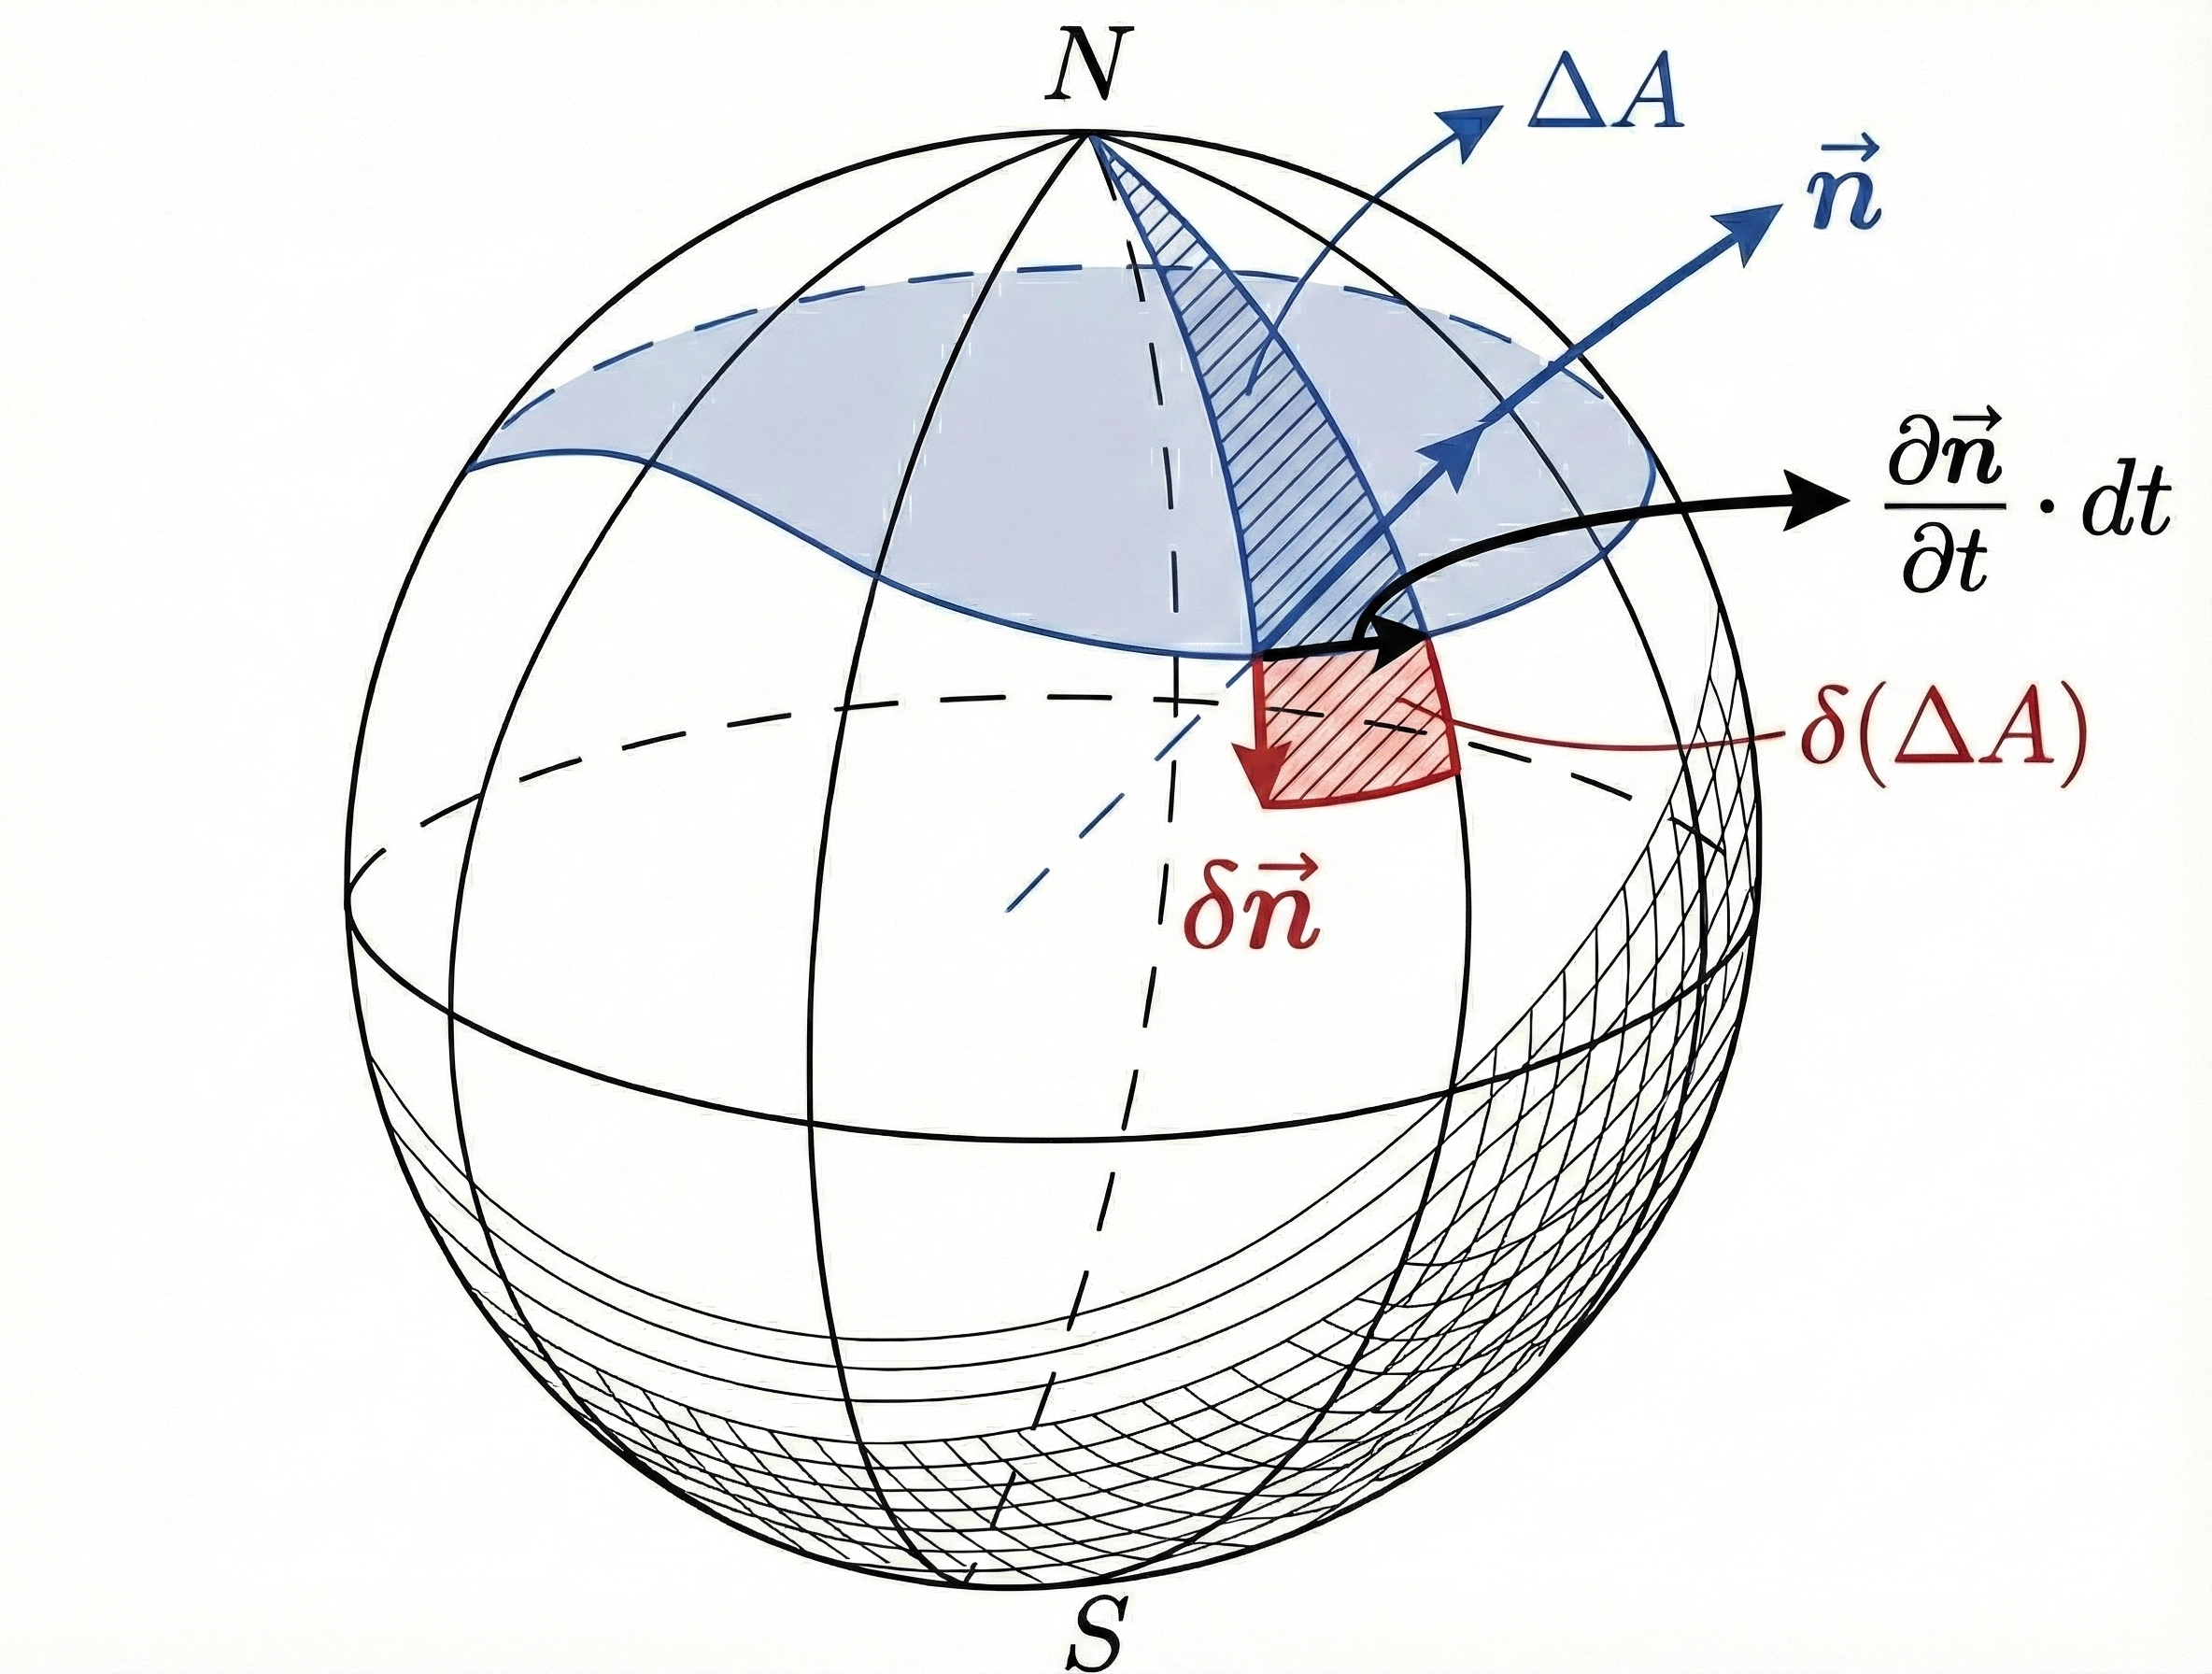
\includegraphics[width=0.5\textwidth]{imgs/SwzVariationDiagram.png}
    \caption{Swz Variation Diagram}
    \label{fig:swz_variation}
\end{figure}

We product $\bm{n}$ on the both sides of the equation :
\begin{equation}
\begin{aligned}
\delta(\Delta A) &= \bm{n} (\delta \bm{n} \times \frac{\partial \bm{n}}{\partial t}) \mathrm{d}t \\
&= - \delta \bm{n} (\bm{n} \times \frac{\partial \bm{n}}{\partial t}) \mathrm{d}t.
\end{aligned}
\end{equation}

Therefore, the variation of the Wess-Zumion part of the action is:
\begin{equation}
\delta (\int \mathrm{d}^d x S_{\mathrm{WZ}}(\bm{n})) 
= \frac{S}{a_0^d} \int \mathrm{d}t \mathrm{d}^d x [\delta \bm{n} \cdot (\bm{n} \times \frac{\partial \bm{n}}{\partial t})]
\end{equation}
This implies the functional derivative is:
\begin{equation}
\frac{\delta S_g}{\delta \bm{n}} = \frac{S}{a_0^d} \cdot (\bm{n} \times \frac{\partial \bm{n}}{\partial t})
\end{equation}

Next, we calculate the variation of energy term:
\begin{equation}
\begin{aligned}
\delta [\int \mathrm{d}^d x \mathrm{d}t (\nabla \bm{n})^2] &= \int \mathrm{d}^d x \mathrm{d}t \frac{1}{2} \delta (\frac{\partial \bm{n}}{\partial x_i})^2 \\
&= \int \mathrm{d}^d x \mathrm{d}t \cdot \sum_i \frac{1}{2} \cdot 2 (\frac{\partial \bm{n}}{\partial x_i}) \cdot \delta (\frac{\partial \bm{n}}{\partial x_i})
\end{aligned}
\end{equation}

And we use the partial integration method:
\begin{equation}
\begin{aligned}
    \int d^d x \sum_i^d 2 \left( \frac{\partial \bm{n}}{\partial x_i} \right) \cdot \delta \left( \frac{\partial \bm{n}}{\partial x_i} \right) 
    &\overset{\frac{\partial \bm{n}}{\partial x_i} = \partial_i \bm{n}}{=\joinrel=\joinrel=} 
    2 \int d^d x \sum_i^d (\partial_i \bm{n}) \cdot \partial_i (\delta \bm{n}) \\
    &= 2 \left\{ \left[ \sum_i^d (\partial_i \bm{n}) \cdot \delta \bm{n} \right] \Bigg|_{\bm{n}_0}^{\bm{n}_N = \bm{n}_0}
    - \int d^d x \sum_i^d \delta \bm{n} \cdot \partial_i^2 \bm{n} \right\} \\
    &= -2 \int d^d x (\nabla^2 \bm{n}) \cdot \delta \bm{n}
\end{aligned}
\end{equation}

So the variation of energy term is
\begin{equation}
\frac{\delta S_e}{\delta \bm{n}} = \frac{|J|S^2}{a_0^{d-2}} (\nabla^2 \bm{n})
\end{equation}
Finally, we calculate the variation of $\lambda$ term:
\begin{equation}
\delta \int \mathrm{d}^d x \mathrm{d}t \frac{\lambda}{2}(\bm{n}^2 - 1) = \int \mathrm{d}^d x \mathrm{d}t \cdot \lambda \bm{n} \delta \bm{n}
\end{equation}
So the variation of $\lambda$ term is:
\begin{equation}
\frac{\delta S_\lambda}{\delta \bm{n}} = \lambda \bm{n}
\end{equation}
Now we can get the total action's variation:
\begin{equation}
\delta S_{\mathrm{tot}} = 0 \implies \frac{S}{a_0^d} (\bm{n} \times \frac{\partial \bm{n}}{\partial t}) + \lambda \bm{n} = - \frac{|J|S^2}{a_0^{d-2}} \nabla^2 \bm{n}.
\end{equation}
To find the value of the Lagrange multiplier, take the dot product of the above equation with $\bm{n}$:
\begin{equation}
    \underbrace{ \frac{S}{a_0^d} \bm{n} \cdot \left( \bm{n} \times \frac{\partial \bm{n}}{\partial t} \right) }_{
        \begin{subarray}{l} 
          = \frac{S}{a_0^d} \frac{\partial \bm{n}}{\partial t} (\bm{n} \times \bm{n}) \\ 
          = 0 
        \end{subarray}
      }
      + \lambda \underbrace{ \bm{n} \cdot \bm{n} }_{=1}
      = - \frac{|J| S^2}{a_0^{d-2}} (\bm{n} \cdot \nabla^2 \bm{n})
\end{equation}
Thus:
\begin{equation}
\lambda = - \frac{|J|S^2}{a_0^{d-2}} (\bm{n} \cdot \nabla^2 \bm{n})
\end{equation}
Now, substitute the $\lambda$ back into equation:
\begin{equation}
\frac{S}{a_0^d} \cdot (\bm{n} \times \frac{\partial \bm{n}}{\partial t}) - [\frac{|J|S^2}{a_0^{d-2}} (\bm{n} \cdot \nabla^2 \bm{n})] \bm{n} = - \frac{|J|S^2}{a_0^{d-2}} \nabla^2 \bm{n}
\end{equation}
Rearrange to group the derivative terms on the right:
\begin{equation}
\frac{S}{a_0^d} (\bm{n} \times \frac{\partial \bm{n}}{\partial t}) = - \frac{|J|S^2}{a_0^{d-2}} [\nabla^2 \bm{n} - (\bm{n} \cdot \nabla^2 \bm{n}) \cdot \bm{n}]
\end{equation}
If we look at: $\bm{n} \times (\bm{n} \times \nabla^2 \bm{n})$:
\begin{equation}
\begin{aligned}
\bm{n} \times (\bm{n} \times \nabla^2 \bm{n}) &= \bm{n} \cdot (\bm{n} \cdot \nabla^2 \bm{n}) - \nabla^2 \bm{n} (\bm{n} \cdot \bm{n}) \\
&= \bm{n} (\bm{n} \cdot \nabla^2 \bm{n}) - \nabla^2 \bm{n}.
\end{aligned}
\end{equation}
So,
\begin{equation}
\frac{S}{a_0^d} (\bm{n} \times \partial_t \bm{n}) = \frac{|J|S^2}{a_0^{d-2}} [\bm{n} \times (\bm{n} \times \nabla^2 \bm{n})]
\end{equation}
Simplified to:
\begin{equation}
\bm{n} \times \frac{\partial \bm{n}}{\partial t} = \bm{n} \times [|J| S a_0^2 (\nabla^2 \bm{n})]
\end{equation}
We can get the Landau-Lifshitz equation:
\begin{equation}
    \colorboxed{
    \frac{\partial \bm{n}}{\partial t} = |J| S a_0^2 (\bm{n} \times \nabla^2 \bm{n}).
    }
\end{equation}

From this equation, we can know that the spins move in a precessional fashion with an angular velocity $\bm{\Omega}$ given by:
\begin{equation}
\bm{\Omega} = -|J|S a_0^2 \nabla^2 \bm{n}.
\end{equation}
The Landau-Lifshitz equations can be solved in the linear regime. Let's parametrize $\bm{n}$ by the components:

\begin{equation}
\bm{n} = \begin{pmatrix} \sigma \\ \bm{\pi} \end{pmatrix} \text{ and } \bm{\pi} = \begin{pmatrix} \pi_1 \\ \pi_2 \end{pmatrix}
\end{equation}
where $\sigma$ and $\pi_i (i=1,2)$ satisfy the constraint:
\begin{equation}
\sigma^2 + \bm{\pi}^2 = 1
\end{equation}
If the system is ordered, $\sigma \sim 1$, $|\bm{\pi}|$ is very small, which means that $\bm{\pi}$ is small fluctuation around the direction of $\sigma$.
In this situation, we can treat $\sigma$ as a constant:
\begin{equation}
\begin{cases}
\sigma \approx 1 \\
\nabla^2 \sigma \approx 0
\end{cases}
\end{equation}
Therefore, we can linearize the Landau-Lifshitz equation:
\begin{equation}
\bm{n} \times \nabla^2 \bm{n} = \begin{pmatrix} \pi_1 \nabla^2 \pi_2 - \pi_2 \nabla^2 \pi_1 \\ -\sigma \nabla^2 \pi_2 \\ \sigma \nabla^2 \pi_1 \end{pmatrix}
\end{equation}
and we remain the one order term :
\begin{equation}
\bm{n} \times \nabla^2 \bm{n} = \begin{pmatrix} 0 \\ -\nabla^2 \pi_2 \\ \nabla^2 \pi_1 \end{pmatrix}
\end{equation}
So the linearizing Landau-Lifshitz equation:
\begin{equation}
\begin{cases}
\partial_t \pi_1 = -|J|S a_0^2 \nabla^2 \pi_2 \\
\partial_t \pi_2 = +|J|S a_0^2 \nabla^2 \pi_1
\end{cases}
\end{equation}

We look for plane wave solutions (spin wave) of the term:
\begin{equation}
\pi_j(\bm{x}, t) = \tilde{\pi}_j e^{\mathrm{i}(\bm{p} \cdot \bm{x} - \omega t)}
\end{equation}
taking derivatives this ansatz converts differential operators into algebraic variables:
\begin{equation}
\begin{cases}
\partial_t \to -\mathrm{i}\omega \\
\nabla^2 \to -|\bm{p}|^2
\end{cases}
\end{equation}
Substituting these into the linearized equations:
\begin{equation}
\begin{cases}
-\mathrm{i}\omega \tilde{\pi}_1 = (|J|S a_0^2 |\bm{p}|^2) \tilde{\pi}_2 \\
-\mathrm{i}\omega \tilde{\pi}_2 = -(|J|S a_0^2 |\bm{p}|^2) \tilde{\pi}_1
\end{cases}
\end{equation}
let $A = |J|S a_0^2 p^2$, the system become:
\begin{equation}
\begin{cases}
-\mathrm{i}\omega \tilde{\pi}_1 - A \tilde{\pi}_2 = 0 \\
A \tilde{\pi}_1 - \mathrm{i}\omega \tilde{\pi}_2 = 0
\end{cases}
\end{equation}
for a non-trivial solution $(\tilde{\pi}_1, \tilde{\pi}_2 \neq 0)$, the determinant of the coefficient matrix must be zero:
\begin{equation}
\begin{vmatrix}
-\mathrm{i}\omega & -A \\
A & -\mathrm{i}\omega
\end{vmatrix} = 0
\end{equation}

we can get:
\begin{equation}
\omega = \pm A.
\end{equation}
So we obtain the dispersion relation for ferromagnetic spin waves:
\begin{equation}
    \colorboxed{
    |\omega| \approx |J|S a_0^2 |\bm{p}|^2
    }
\end{equation}
We find that the frequency of the low-energy excitations of a quantum ferromagnetic scales as the square of the momentum.

\begin{figure}[htbp]
    \centering
    \begin{tikzpicture}[
        % 定义样式
        scale=0.7,
        >=Stealth, % 箭头样式
        axis/.style={dashed, thin, darkgray}, % H场轴线样式
        spin/.style={thick, blue, ->}, % 自旋磁矩M样式
        orbit/.style={
            black, thin,
            postaction={decorate},
            decoration={
                markings,
                mark=at position 0.6 with {\arrow{>}} % 在椭圆轨迹上添加方向箭头
            }
        }
    ]

    % 循环生成12个图 (索引 k 从 0 到 11)
    \foreach \k in {0,...,11} {
        
        % --- 计算逻辑 ---
        % 1. 计算行列位置 (每行6个)
        \pgfmathsetmacro{\row}{int(\k / 6)}
        \pgfmathsetmacro{\col}{int(mod(\k, 6))}
        
        % 2. 定义每个子图的偏移量 (X间距3.3, Y间距4.5)
        \pgfmathsetmacro{\xshift}{\col * 3.3}
        \pgfmathsetmacro{\yshift}{-\row * 4.5}
        
        % 3. 计算旋转角度
        % 图片中每个相位增加 2pi/11。
        % 360度 / 11 ≈ 32.72度
        % 我们设定起始角度为 -20度以匹配图片的视觉效果(Phase 0指向右下方)
        \pgfmathsetmacro{\angledeg}{-30 + \k * (360/11)}
        
        % --- [新增] 绘制红色波形连线 ---
        % 只有当不是每行的第一个元素时,才连接前一个点
        \ifnum\col>0
            % 计算前一个点的参数
            \pgfmathsetmacro{\prevK}{int(\k-1)}
            \pgfmathsetmacro{\prevAngle}{-30 + \prevK * (360/11)}
            \pgfmathsetmacro{\prevXShift}{(\col-1) * 3.3}
            
            % 计算前一个点的绝对坐标
            \pgfmathsetmacro{\prevTipX}{\prevXShift + 1.0 * cos(\prevAngle)}
            \pgfmathsetmacro{\prevTipY}{\yshift + 1.5 + 0.4 * sin(\prevAngle)}
            
            % 计算当前点的绝对坐标
            \pgfmathsetmacro{\currTipX}{\xshift + 1.0 * cos(\angledeg)}
            \pgfmathsetmacro{\currTipY}{\yshift + 1.5 + 0.4 * sin(\angledeg)}
            
            % 绘制红色虚线连接
            \draw[red, dashed, thick] (\prevTipX, \prevTipY) -- (\currTipX, \currTipY);
        \fi

        % 4. 标签文本逻辑
        \pgfmathsetmacro{\numerator}{int(\k * 2)}
        \def\phasetext{Phase $= \frac{\numerator\pi}{11}$}
        
        % 特殊情况处理:第一个和最后一个显示为 0
        \ifnum\k=0 \def\phasetext{Phase $= 0$} \fi
        \ifnum\k=11 \def\phasetext{Phase $= 0$} \fi

        % --- 开始在指定位置绘图 ---
        \begin{scope}[shift={(\xshift, \yshift)}]
            
            % 定义关键坐标
            \coordinate (origin) at (0,0);       % 圆锥顶点
            \coordinate (center) at (0, 1.5);    % 椭圆中心 (圆锥底部中心)
            \coordinate (top) at (0, 2.2);       % H轴顶部

            % 1. 绘制椭圆轨迹 (进动轨迹)
            % 椭圆长轴1.0,短轴0.4
            \draw[orbit] (center) ellipse (1.0 and 0.4);

            % 2. 绘制 H 场 (中轴线)
            % 也就是圆锥的中轴,用虚线表示
            \draw[axis] (origin) -- (center);
            \draw[axis, ->] (center) -- (top);
            
            % 仅在第一个图中标注 H 向量
            \ifnum\k=0
                \node[left, font=\footnotesize] at (0, 2.0) {$\vec{H}$};
            \fi

            % 3. 绘制 M 磁矩 (自旋向量)
            % 计算箭头在椭圆上的落点
            % x = x_radius * cos(angle)
            % y = y_center + y_radius * sin(angle)
            \pgfmathsetmacro{\tipx}{1.0 * cos(\angledeg)}
            \pgfmathsetmacro{\tipy}{1.5 + 0.4 * sin(\angledeg)}
            \coordinate (tip) at (\tipx, \tipy);

            % 画蓝色箭头
            \draw[spin] (origin) -- (tip);

            % 仅在第一个图中标注 M 向量
            \ifnum\k=0
                \node[right, blue, font=\footnotesize] at (tip) {$\vec{M}$};
            \fi
            
            % 4. 绘制底部的 Phase 标签
            \node[below, font=\small] at (0, -0.2) {\phasetext};

        \end{scope}
    }

    \end{tikzpicture}
    \caption{Schematic diagram of spin wave phase variation}
\end{figure}

\section{Quantum Antiferromagnetic of one-dimension}

Consider a spin chain with an even number of sites $N$; we can write down the action of it ($J=|J|$):
\begin{equation}
    \label{eq:action_afm}
    S_M[\bm{n}] = S \sum_{i}^N S_{WZ}[\bm{n}] - \int \mathrm{d}t \sum_{i}^N J S^2 \bm{n}(i,t) \cdot \bm{n}(i+1, t)
\end{equation}
where we have assumed periodic boundary conditions.

\begin{figure}[htbp]
    \centering
    \begin{tikzpicture}[
        x=1.2cm, 
        y=1.2cm, 
        every node/.style={font=\sffamily},
        thick
    ]

        % --- 2. Styles Definition ---
        \tikzset{
            site/.style={circle, fill=black, inner sep=2.5pt},
            arrow/.style={->, >={Stealth[round, length=3mm, width=2mm]}, very thick},
            label text/.style={below=0.4cm, font=\large\itshape}
        }

        % --- 3. Drawing the Left Side (Start) ---
        % Site 1
        \node[site] (s1) at (0,0) {};
        \node[label text] at (0,0) {$1$};
        % Let's assume the first spin is Up -> RED
        \draw[arrow, red] (0, 0.4) -- (0, 1.0);

        % Ellipsis (...)
        \draw[dashed, very thick] (0.8, 0) -- (2.2, 0);
        \node[below=0.1cm] at (1.5, 0) {$\dots$};


        % --- 4. Drawing the Middle Sequence ---
        % Pattern from image: 
        % Arrow 1: Up (no label)
        % Arrow 2: Down (label i-1)
        % Arrow 3: Up (label i)
        % Arrow 4: Down (label i+1)
        % Arrow 5: Up (label i+2)
        % Arrow 6: Down (label i+3)
        % Arrow 7: Up (no label)
        % Arrow 8: Down (no label)
        
        % Define starting x position for the middle block
        \def\startx{3}

        % Loop to generate the middle section
        % Format: offset / direction (1=up, -1=down) / label
        \foreach \offset / \dir / \lab in {
            0/1/,          % Up, no label
            1/-1/i-1,      % Down, i-1
            2/1/i,         % Up, i
            3/-1/i+1,      % Down, i+1
            4/1/i+2,       % Up, i+2
            5/-1/i+3,      % Down, i+3
            6/1/,          % Up, no label
            7/-1/          % Down, no label
        } {
            \coordinate (pos) at (\startx + \offset, 0);
            
            % Draw the site dot
            \node[site] at (pos) {};
            
            % Draw the Label (if present)
            \ifx\lab\empty
            \else
                \node[label text] at (pos) {$\lab$};
            \fi
            
            % Draw the Arrow
            \ifnum\dir=1
                % Up Arrow -> RED
                \draw[arrow, red] (\startx + \offset, 0.4) -- ++(0, 0.7);
            \else
                % Down Arrow -> BLUE
                \draw[arrow, blue] (\startx + \offset, 1.1) -- ++(0, -0.7);
            \fi
        }

        % --- 5. Drawing the Right Side (End) ---
        % Ellipsis (...)
        \draw[dashed, very thick] (\startx + 7.8, 0) -- (\startx + 9.2, 0);
        \node[below=0.1cm] at (\startx + 8.5, 0) {$\dots$};

        % Site N
        \coordinate (end) at (\startx + 10, 0);
        \node[site] at (end) {};
        \node[label text] at (end) {$N$};
        % Assuming even number and alternating pattern finishing (Down) -> BLUE
        \draw[arrow, blue] (\startx + 10, 1.1) -- ++(0, -0.7);

        % Bottom reference dashes (optional, imitating the sketchy lines under labels in the image)
        % \draw[gray, thin, dashed] (-0.5, -0.8) -- (14, -0.8);

    \end{tikzpicture}
    \caption{Illustration of a 1D spin chain with an even number of sites, showing alternating spins around site $i$.}
    \label{fig:spin_afm_diagram}
\end{figure}


Since we expect to be close to a N\'{e}el state, we will stagger the configuration:
\begin{equation}
    \label{eq:staggered_configuration}
    \bm{n}(j) \to (-1)^j \bm{n}(j)
\end{equation}

On a bipartite lattice, the substitution of \cref{eq:staggered_configuration} into \cref{eq:action_afm} will change the sign of the exchange term of the action to a ferromagnetic:
\begin{equation}
S_M[\bm{n}] = S \sum_{i}^N (-1)^i S_{WZ}[\bm{n}(i)] - \frac{|J|S^2}{2} \int \mathrm{d}t \sum_{i=1}^N (-1)^i \bm{n}(i,t) \cdot (-1)^{i+1} \bm{n}(i+1,t)
\end{equation}
so the energy term become to:
\begin{equation}
S_e = \frac{|J|S^2}{2} \int \mathrm{d}t \sum_{i=1}^N \bm{n}(i,t) \bm{n}(i+1,t)
\end{equation}
which is similar to ferromagnetic.
But the Wess-Zumino terms become staggered under the replacement of \cref{eq:staggered_configuration}.
Thus, it is the Wess-Zumino term, a purely quantum-mechanical effect, 
which will distinguish ferromagnets from antiferromagnets.

As antiferromagnetic, we can split $\bm{n}$ into a slowly varying piece $\bm{m}$ plus a small rapidly varying part $a_0 \bm{l}$, so:
\begin{equation}
\bm{n}(i) = \bm{m}(i) + (-1)^i a_0 \bm{l}(i)
\end{equation}

The constraint $|\bm{n}|^2=1$ and requirement that $\bm{m}$ should obey the same constraint, and demand that $\bm{m}$ and $\bm{l}$ be orthogonal vector:
\begin{equation}
\begin{cases}
|\bm{m}|^2 = 1 \\
\bm{m} \cdot \bm{l} = 0
\end{cases}
\end{equation}
The Wess-Zumino terms are rewritten as:
\begin{equation}
S \sum_i^N (-1)^i S_{WZ}[\bm{n}(i)] = S \sum_{r=1}^{N/2} \{ S_{WZ}[\bm{n}(2r)] - S_{WZ}[\bm{n}(2r-1)] \}
\end{equation}

\begin{figure}[htbp]
    \centering
    \resizebox{\textwidth}{!}{%
    \begin{tikzpicture}[
        % Spin styles
        spin/.style={circle, inner sep=0pt, minimum size=0.8cm, draw=none},
        % Spin Down (Blue ball, down arrow)
        spin down/.style={spin, fill=blue!60, 
            path picture={
                \draw[->, white, ultra thick, >=Stealth] (0, 0.25) -- (0, -0.25);
            }
        },
        % Spin Up (Red ball, up arrow)
        spin up/.style={spin, fill=red!60, 
            path picture={
                \draw[->, white, ultra thick, >=Stealth] (0, -0.25) -- (0, 0.25);
            }
        },
        % Dimer style
        dimer/.style={draw, ellipse, inner sep=5pt, thick, minimum height=1.6cm},
        % Label style
        every label/.style={font=\large} 
    ]

        % Define spacing - Adjusted to separate dimers more
        \def\spinsep{1.6}  % 略微增加二聚体内部两个自旋的距离
        \def\dimersep{4.5} % 大幅增加二聚体之间的距离,防止重合

        % --- Group 1 (1, 2) ---
        \node[spin down, label=below:$1$] (s1) at (0,0) {};
        \node[spin up, label=below:$2$] (s2) at (\spinsep,0) {};
        \node[dimer, fit=(s1)(s2)] (d1) {};

        % --- Group 2 (3, 4) ---
        \begin{scope}[shift={(\dimersep, 0)}]
            \node[spin down, label=below:$3$] (s3) at (0,0) {};
            \node[spin up, label=below:$4$] (s4) at (\spinsep,0) {};
            \node[dimer, fit=(s3)(s4)] (d2) {};
        \end{scope}

        % --- Group 3 (5, 6) ---
        \begin{scope}[shift={(2*\dimersep, 0)}]
            \node[spin down, label=below:$5$] (s5) at (0,0) {};
            \node[spin up, label=below:$6$] (s6) at (\spinsep,0) {};
            \node[dimer, fit=(s5)(s6)] (d3) {};
        \end{scope}

        % --- Group r (2r-1, 2r) ---
        % Place at 4.5 * dimersep to leave a gap
        \begin{scope}[shift={(4.5*\dimersep, 0)}]
            \node[spin down, label=below:$2r-1$] (sr1) at (0,0) {};
            \node[spin up, label=below:$2r$] (sr2) at (\spinsep,0) {};
            \node[dimer, fit=(sr1)(sr2)] (dr) {};
        \end{scope}

        % --- Group N (N-1, N) ---
        % Place at 7.0 * dimersep to leave another gap
        \begin{scope}[shift={(7.0*\dimersep, 0)}]
            \node[spin down, label=below:$N-1$] (sN1) at (0,0) {};
            \node[spin up, label=below:$N$] (sN2) at (\spinsep,0) {};
            \node[dimer, fit=(sN1)(sN2)] (dN) {};
        \end{scope}

        % --- Ellipses ---
        % Draw ellipsis exactly between d3 and dr
        \path (d3) -- node[auto=false, font=\huge] {$\cdots$} (dr);
        
        % Draw ellipsis exactly between dr and dN
        \path (dr) -- node[auto=false, font=\huge] {$\cdots$} (dN);

    \end{tikzpicture}
    } % end resizebox
    \caption{Schematic of 1D Antiferromagnetic Spin Chain}
    \label{fig:afm_chain}
\end{figure}


By making use of the approximation:
\begin{equation}
\begin{aligned}
\bm{n}(2r) - \bm{n}(2r-1) &= \bm{m}(2r) - \bm{m}(2r-1) + a_0 [\bm{l}(2r) + \bm{l}(2r-1)] \\
&\approx a_0 \left[ \frac{\partial \bm{m}(2r)}{\partial x} + 2 \bm{l}(2r) \right] + O(a_0^2)
\end{aligned}
\end{equation}
So the geometric term becomes (use the similar method of area variation, see \cref{fig:antiferromagnetic_variation})
\begin{equation}
\begin{aligned}
S \sum_r^N (-1)^i S_{WZ}[\bm{n}(i)] 
&\approx S \sum_{r=1}^{N/2} (\bm{n}(2r) - \bm{n}(2r-1)) [\bm{n}(2r) \times \frac{\partial \bm{n}(2r)}{\partial t}] \\
&\approx S \sum_{r=1}^{N/2} a_0 \left[ \frac{\partial \bm{m}(2r)}{\partial x} + 2 \bm{l}(2r) \right] \left[ \bm{m}(2r) \times \frac{\partial \bm{m}(2r)}{\partial t} \right]
\end{aligned}
\end{equation}

\begin{figure}
    \centering
    \includegraphics[width=0.5\textwidth]{imgs/AntiferromagneticVariationDiagram.png}
    \caption{Antiferromagnetic Variation Diagram}
    \label{fig:antiferromagnetic_variation}
\end{figure}

Using continuum limit ($a_0 \to 0$):
\begin{equation}
\begin{aligned}
\lim_{a_0 \to 0} S_g 
&\approx \frac{S}{2} \sum_{r=1}^N (\dots) \quad (\text{periodic boundary conditions}) \\
&= \frac{S}{2} \int \mathrm{d}x \mathrm{d}t (\partial_x \bm{m} + 2 \bm{l}) \cdot (\bm{m} \times \partial_t \bm{m})
\end{aligned}
\end{equation}

Thus, it can be simplified to:
\begin{equation}
S_g \approx \frac{S}{2} \int \mathrm{d}x \mathrm{d}t \cdot \bm{m} (\partial_t \bm{m} \times \partial_x \bm{m}) + S \int \mathrm{d}x \mathrm{d}t \bm{l} (\bm{m} \times \partial_t \bm{m})
\end{equation}
This term comes from alternating sum of WZ terms.
Similarly, the continuum limit of the energy terms can also be found to be given by:
\begin{equation}
\begin{aligned}
&\lim_{a_0 \to 0} \frac{|J|S^2}{2} \int \mathrm{d}t \sum_{i=1}^N \bm{n}(i,t) \bm{n}(i+1,t) \\
\xrightarrow{\text{drop global phase}} &\lim_{a_0 \to 0} \frac{-|J|S^2}{2} \int \mathrm{d}t \sum_{i=1}^N [\bm{n}(i+1,t) - \bm{n}(i,t)]^2 \\
&\approx \frac{-|J|S^2}{2} \int \mathrm{d}t \sum_i [ (\bm{m}(i+1) - \bm{m}(i)) + a_0 \bm{l}(i+1) + a_0 \bm{l}(i) ]^2 \\
&\approx \frac{-|J|S^2}{2} \int \mathrm{d}t \sum_i a_0^2 (\frac{\Delta \bm{m}}{a_0} + 2\bm{l})^2 \\
&= \frac{-|J|S^2}{2} \int \mathrm{d}t a_0 \int \mathrm{d}x [ (\partial_x \bm{m})^2 + \underbrace{4 \frac{\Delta \bm{m}}{a_0} \cdot \bm{l}}_{=0} + 4\bm{l}^2 ] \\
&= \frac{-|J|S^2 a_0}{2} \int \mathrm{d}t \mathrm{d}x [ (\partial_x \bm{m})^2 + 4\bm{l}^2 ]
\end{aligned}
\end{equation}
So the total Lagrangian density involving both the order parameter $\bm{m}$ and $\bm{l}$:
\begin{equation}
\mathcal{L}_M(\bm{m}, \bm{l}) = -2 a_0 |J| S^2 \bm{l}^2 + S \bm{l} (\bm{m} \times \partial_t \bm{m}) - \frac{a_0 |J| S^2}{2} (\partial_x \bm{m})^2 + \frac{S}{2} \bm{m} \cdot (\partial_t \bm{m} \times \partial_x \bm{m})
\end{equation}
where $\bm{m}$ is the order parameter field and $\bm{l}$ roughly represents the average spin field.

The Lagrangian has a quadratic term for $\bm{l}$:
\begin{equation}
\mathcal{L}_{\bm{l}} = -2 a_0 |J| S^2 \bm{l}^2 + S (\bm{m} \times \partial_t \bm{m}) \bm{l}.
\end{equation}
To integrate out $\bm{l}$, we minimize the action with respect to $\bm{l}$:
\begin{equation}
\frac{\partial \mathcal{L}_{\bm{l}}}{\partial \bm{l}} = -4 a_0 |J| S^2 \bm{l} + S (\bm{m} \times \partial_t \bm{m}) = 0
\end{equation}
so we solve for $\bm{l}$:
\begin{equation}
\bm{l} = \frac{1}{4 a_0 |J| S} (\bm{m} \times \partial_t \bm{m})
\end{equation}
Now we subsitute the expression for $\bm{l}$ found above back into $\mathcal{L}_{\bm{l}}$:
\begin{equation}
\begin{aligned}
\mathcal{L}_{\bm{l}}^{\text{eff}} &= \frac{1}{8 a_0 |J|} (\bm{m} \times \partial_t \bm{m})^2 \quad (\bm{m} \perp \partial_t \bm{m} \text{ because } \bm{m} \text{ is on the sphere}) \\
&= \frac{1}{8 a_0 |J|} (\partial_t \bm{m})^2
\end{aligned}
\end{equation}
Final we can combine the new term with original term that do not depend on $\bm{l}$:
\begin{equation}
    \label{eq:lagrangian_density}
    \begin{aligned}
    \mathcal{L}(\bm{m}) &= \frac{1}{8 a_0 J} (\partial_t \bm{m})^2 - \frac{a_0 J S^2}{2} (\partial_x \bm{m})^2 + \frac{S}{2} \bm{m} (\partial_t \bm{m} \times \partial_x \bm{m}) \\
    &= \frac{1}{2g} \left[ \frac{1}{v_s} (\partial_t \bm{m})^2 - v_s (\partial_x \bm{m})^2 \right] + \underbrace{\frac{\theta}{8\pi} \epsilon_{\mu\nu} \bm{m} (\partial_\mu \bm{m} \times \partial_\nu \bm{m})}_{\text{Einstein summation}}
    \end{aligned}
    \end{equation}
where $g$ and $v_s$ are respectively the coupling constant and spin-wave velocity:
\begin{equation}
\begin{cases}
g = \frac{2}{S} \\
v_s = 2 a_0 |J| S
\end{cases}
\end{equation}

The last term in \cref{eq:lagrangian_density} has topological significance. 
We have chosen the normalization so that the coupling constant $\theta$ is given by:
\begin{equation}
\theta = 2 \pi S
\end{equation}
The tensor $\epsilon_{\mu\nu}$ is the usual Levi-Civita antisymmetric tensor in two dimensions 
($\mu,\nu=t,x(t \to 0, x \to 1)$):
\begin{equation}
\epsilon_{\mu\nu} = \begin{cases}
1 & (\mu,\nu) = (0,1) \\
-1 & (\mu,\nu) = (1,0) \\
0 & \text{otherwise}.
\end{cases}
\end{equation}
The result is the Lagrangian density of non-linear sigma model.

\section{The role of topological term.}

Go back to Euclidean spacetime ($\mathrm{i} S_M \to -S_E$):
\begin{equation}
\mathrm{i} S_M = \mathrm{i} \int \mathrm{d}t \mathrm{d}x \mathcal{L}_M [\bm{m}(t,x)] 
= - \int \mathrm{d}\tau \mathrm{d}x \mathcal{L}_E [\bm{m}(\tau,x)]
\end{equation}
So we can get the Lagrangian density $\mathcal{L}_E$ of Euclidean sector ($x_2 = \mathrm{i}t = \mathrm{i}x_0$)
\begin{equation}
    \colorboxed{
    \mathcal{L}_E = \frac{1}{2g} [(\partial_1 \bm{m})^2 + (\partial_2 \bm{m})^2] + 
    \frac{\mathrm{i}\theta}{8\pi} \epsilon_{ij} \bm{m} \cdot (\partial_i \bm{m} \times \partial_j \bm{m})
    }
\end{equation}
where $i,j = 1,2$.

We now define the Pontryagin index or topological charge (or winding number) $\mathcal{Q}$ 
of the Euclidean space spin configuration $\{\bm{m}(\bm{x})\}$ by the following expression:
\begin{equation}
    \colorboxed{
    \begin{aligned}
    \mathcal{Q} &= \frac{1}{8\pi} \int \mathrm{d}^2x \, \epsilon_{ij} \bm{m} (\partial_i \bm{m} \times \partial_j \bm{m}) \\
    &= \frac{1}{4\pi} \int \mathrm{d}^2x \, \bm{m} (\partial_1 \bm{m} \times \partial_2 \bm{m})
    \end{aligned}
    }
\end{equation}
We impose the boundary condition that the Euclidean action be finite. This is equivalent to the requirement that asymptotically $\bm{m}$ becomes a constant vector $\bm{m}_0$ at spatial-time infinity:
\begin{equation}
\lim_{|\bm{x}|\to\infty} \bm{m}(\bm{x}) = \bm{m}_0
\end{equation}
Thus, the 2D Euclidean space-time is isomorphic to a sphere $S_2$ since the fields are identified with $\bm{m}_0$ at the point of infinity.
However, the order parameter manifold ("target space") is also isomorphic to a sphere $S_2$, 
since the constraint $\bm{m}^2=1$ has to be satisfied everywhere(see figure \ref{fig:topological_mapping}).

% 设置随机种子以保证每次编译得到的内部自旋形态一致
\pgfmathsetseed{42}
\begin{figure}[htbp]
    \centering
    \begin{tikzpicture}[
        >=Latex, 
        font=\small,
        % Define styles for consistency
        axis_style/.style={thin, gray!50},
        vector_style/.style={->, thick, color=black!80, line cap=round},
        sphere_style/.style={circle, draw=black, thick, minimum size=3cm},
        label_style/.style={align=center, font=\footnotesize\bfseries}
    ]

        % 定义布局坐标
        % POS_TOP 的 y 坐标为 6.0
        \coordinate (POS_TOP) at (3.5, 6.0);   % 顶部中心 (网格)
        \coordinate (POS_LEFT) at (0, 0);      % 左下 (Base Space)
        \coordinate (POS_RIGHT) at (8, 0);     % 右下 (Target Space)

        % ==========================================
        % STAGE 1: 2D Euclidean Space-time (TOP)
        % ==========================================
        \begin{scope}[shift={($(POS_TOP) + (-2.0, -1.0)$)}, scale=0.55]
            
            % --- 用户提供的代码逻辑 ---
            \tikzset{
                x={(1cm,0cm)},
                y={(0.8cm,0.5cm)}, 
                z={(0cm,1cm)}
            }
            \def\Nx{6} 
            \def\Ny{5} 
            \def\ArrowLen{0.8}

            % 1. 绘制网格
            \foreach \y in {0,...,\Ny} {
                \draw[gray!80, thin] (0, \y, 0) -- (\Nx, \y, 0);
            }
            \foreach \x in {0,...,\Nx} {
                \draw[gray!80, thin] (\x, 0, 0) -- (\x, \Ny, 0);
            }

            % 2. 绘制自旋
            \foreach \y in {\Ny,...,0} {
                \foreach \x in {0,...,\Nx} {
                    \pgfmathparse{int(\x==0 || \x==\Nx || \y==0 || \y==\Ny)}
                    \let\isBoundary\pgfmathresult
                    \ifnum\isBoundary=1
                        \draw[->, thick, color=black!80] (\x,\y,0) -- ++(0,0,\ArrowLen);
                    \else
                        \pgfmathsetmacro{\rx}{rand*0.35}
                        \pgfmathsetmacro{\ry}{rand*0.35}
                        \draw[->, thick, color=black!80] (\x,\y,0) -- ++(\rx,\ry,\ArrowLen);
                    \fi
                }
            }
            % --- 结束 ---
            
            % 定义一个从网格引出箭头的锚点
            \coordinate (grid_anchor) at (1, 0, 0); 
        \end{scope}
        
        % Label for Stage 1 (Top)
        \node[label_style] at ($(POS_TOP) + (0, -2.0)$) {2D Euclidean\\Space-time};


        % ==========================================
        % STAGE 2: Base Space Sphere (BOTTOM LEFT)
        % ==========================================
        \begin{scope}[shift={(POS_LEFT)}]
            % Sphere outline
            \shade[ball color=white, opacity=0.2] (0,0) circle (1.5);
            \draw[thick] (0,0) circle (1.5);
            
            % Grid lines
            \draw[gray] (-1.5,0) arc (180:360:1.5 and 0.5);
            \draw[gray, dashed] (1.5,0) arc (0:180:1.5 and 0.5);
            \draw[gray] (0,1.5) arc (90:270:0.5 and 1.5);
            \draw[gray, dashed] (0,-1.5) arc (-90:90:0.5 and 1.5);
            
            % Vectors
            \foreach \angle in {0, 45, ..., 315} {
                \draw[vector_style] (\angle:1.5) -- (\angle:1.9);
            }
            \draw[vector_style] (0.5, 0.5) -- (0.8, 0.8);
            \draw[vector_style] (-0.3, 0.6) -- (-0.5, 1.0);
            \draw[vector_style] (0.2, -0.8) -- (0.3, -1.2);
            
            % Point x
            \coordinate (x_point) at (45:1.5); 
            % 【修改】调整标签位置到点的右下方 (north west anchor),避免与上方箭头重叠
            \filldraw[black] (x_point) circle (2pt) node[anchor=north west, xshift=2pt, yshift=20pt] {$\bm{x}$};
            
            % Arrow Anchor (Top of sphere)
            \coordinate (sphere1_top) at (0, 1.6);
        \end{scope}

        % Label for Stage 2
        \node[label_style, yshift=-2.2cm] at (POS_LEFT) {Base Space ($S^2$)};


        % ==========================================
        % ARROW 1: Compactification (Top -> Left)
        % ==========================================
        \draw[->, thick, shorten >=2pt] (grid_anchor) to[out=-90, in=70] 
            node[midway, left, align=right, font=\scriptsize, xshift=-2pt] {Isomorphic to $S^2$} 
            (sphere1_top);


        % ==========================================
        % STAGE 3: Target Space Sphere (BOTTOM RIGHT)
        % ==========================================
        \begin{scope}[shift={(POS_RIGHT)}]
            % Sphere outline
            \shade[ball color=white, opacity=0.2] (0,0) circle (1.5);
            \draw[thick] (0,0) circle (1.5);
            
            % Grid lines
            \draw[gray] (-1.5,0) arc (180:360:1.5 and 0.5);
            \draw[gray, dashed] (1.5,0) arc (0:180:1.5 and 0.5);
            \draw[gray] (0,1.5) arc (90:270:0.5 and 1.5);
            \draw[gray, dashed] (0,-1.5) arc (-90:90:0.5 and 1.5);
            
            % Target point
            \coordinate (m_point) at (-0.5, 0.8);
            \filldraw[black] (m_point) circle (2pt) node[anchor=west] {$\bm{m}$};
            \draw[vector_style] (0,0) -- (m_point);
            
            % Arrow Anchor (Left side of sphere)
            \coordinate (sphere2_left) at (-1.6, 0);
        \end{scope}

        % Label for Stage 3
        \node[label_style, yshift=-2.2cm] at (POS_RIGHT) {Target Space ($S^2$)\\Order Parameter Manifold};


        % ==========================================
        % ARROW 2: Mapping (Left -> Right)
        % ==========================================
        \draw[->, thick] (x_point) to[bend left=30] 
            node[midway, above] {$\bm{m}(\bm{x})$} 
            (7.0, 1.0); % Direct coordinate near target sphere

    \end{tikzpicture}
    \caption{Topological mapping from 2D Euclidean space-time to the base space $S^2$ and the target space $S^2$.}
    \label{fig:topological_mapping}
\end{figure}

The topological charge $\mathcal{Q}$ is in the sense that it counts how many times the spin configuration $\bm{m}$ has wrapped around the sphere $S_2$.

So the topological term of action is:
\begin{equation}
    \colorboxed{
    S_{\text{top}} = \mathrm{e}^{\mathrm{i} \cdot 2\pi S \mathcal{Q}} = (-1)^{2S\mathcal{Q}}
    }
\end{equation}
Thus:
\begin{equation}
\mathrm{e}^{\mathrm{i} \cdot 2\pi S \mathcal{Q}} = \begin{cases}
1 & \text{for } S=1,2 \dots (\text{integer spin}) \\
(-1)^{\mathcal{Q}} & \text{for } S=\frac{1}{2}, \frac{3}{2}, \dots (\text{half-odd-integer})
\end{cases}
\end{equation}

We can see that:
\begin{enumerate}[(1)]
    \item $S$ is an integer: the spin chain is described at low energies by the standard non-linear sigma model, without a topological term.
    \item $S$ is half integral $S$: each topological class contributes to the weight of the integral with a sign that is positive (negative) if the winding number $\mathcal{Q}$ is even (odd)
\end{enumerate}

The integer- and half-integer-spin chains fall in different universality classes. We will now see that this property implies a very important result, known as Haldane's conjecture, that states that the integer-spin chains are massive (have an energy gap), whereas the half-integer-spin chains are massless as in the spin one-half case.